Hasta ahora hemos visto cómo la robótica dio sus primeros pasos tras la concepción de los laboratorios de Inteligencia Artificial por todo el mundo, con lo que se produjo un boom en las técnicas y el desarrollo de la robótica. No se le escapará a nadie que actualmente, a la cabeza de la robótica, podemos encontrar ciertas secciones o categorías que se están desarrollando por encima del resto ya sea por su utilidad, por lo vistosos que son o por el simple hecho de buscar un desarrollo en dicho campo. Estas categorías podrían ser: los robots usados en el espacio o expediciones espaciales, los robots usados en la industria militar, los robots diseñados mediante la IA para algún tipo de tarea concreta o los robots que imitan cualidades humanas.

\vspace{10px}

A continuación trataremos de discutir el actual estado de los robots en estas categorías.

\subsubsection{NASA}
Dentro del panorama aeroespacial la agencia que lidera actualmente el desarrollo en la exploración fuera de la Tierra es la NASA. Gracias a esto la agencia espacial estadounidense ha desarrollado un programa de robótica muy amplio y robusto, con robots que van desde la asistencia en viajes espaciales hasta exploración del espacio, telescopios o robots usados en exploraciones planetarias.

\vspace{10px}

Entre los robots diseñados por la NASA no sólo los hay pensados para la exploración de planetas, también se han ideados robots de asistencia para los astronautas. En este grupo de robots podemos meter a la serie Robonaut con las dos versiones desarrolladas hasta el momento. Esta gama de robots están pensados para la asistencia tanto dentro de la nave espacial como fuera de la misma, por ejemplo en tareas de reparación o acoplamiento de módulos. El primer modelo, el Robonaut 1 o R1 nunca llegó al espacio, si no se que empleó como un primer prototipo para estudio y desarrollo. El robot consistía de un torso con forma humana y con la parte de abajo intercambiable, de esta forma se podía adecuar el mismo para la exploración de planetas o colocarle módulos como el Zero-G Leg, pensado para poder engancharse a las barras exteriores que se le suelen colocar a los módulos, naves y estaciones espaciales para facilitar el desplazamiento de los astronautas por el exterior de las mismas (en esta misma línea la NASA tiene un concepto de robot llamado Spidernaut). De esta manera se demostraba que este robot, si se diseñara de forma adecuada, sería útil en misiones de reparación en el exterior de las naves o de asistencia. En su segunda versión el robot mejoró todas sus capacidades y el diseño se convirtió realmente en algo funcional siendo lanzado en 2011 a la ISS (Estación Espacial Internacional). El primer modelo que se envió a la estación no era capaz de moverse pero sí de llevar cosas y mover sus brazos de forma que era útil para sostener cosas como herramientas o moverlas de un sitio a otro con la rotación del torso. Tras ese paso se enviaron a la ISS piernas y módulos extra al robot de forma que ahora ya es capaz de moverse dentro de la estación y es capaz de ver y analizar su entorno. Por el momento no se ha conseguido presurizar el cuerpo lo suficiente como para poder emplearlo en misiones fuera de la estación. Actualmente esta es la línea de desarrollo del robot tanto para misiones fuera de la estación como para misiones de exploración del espacio profundo.

\begin{figure}[!h]
	\centering
	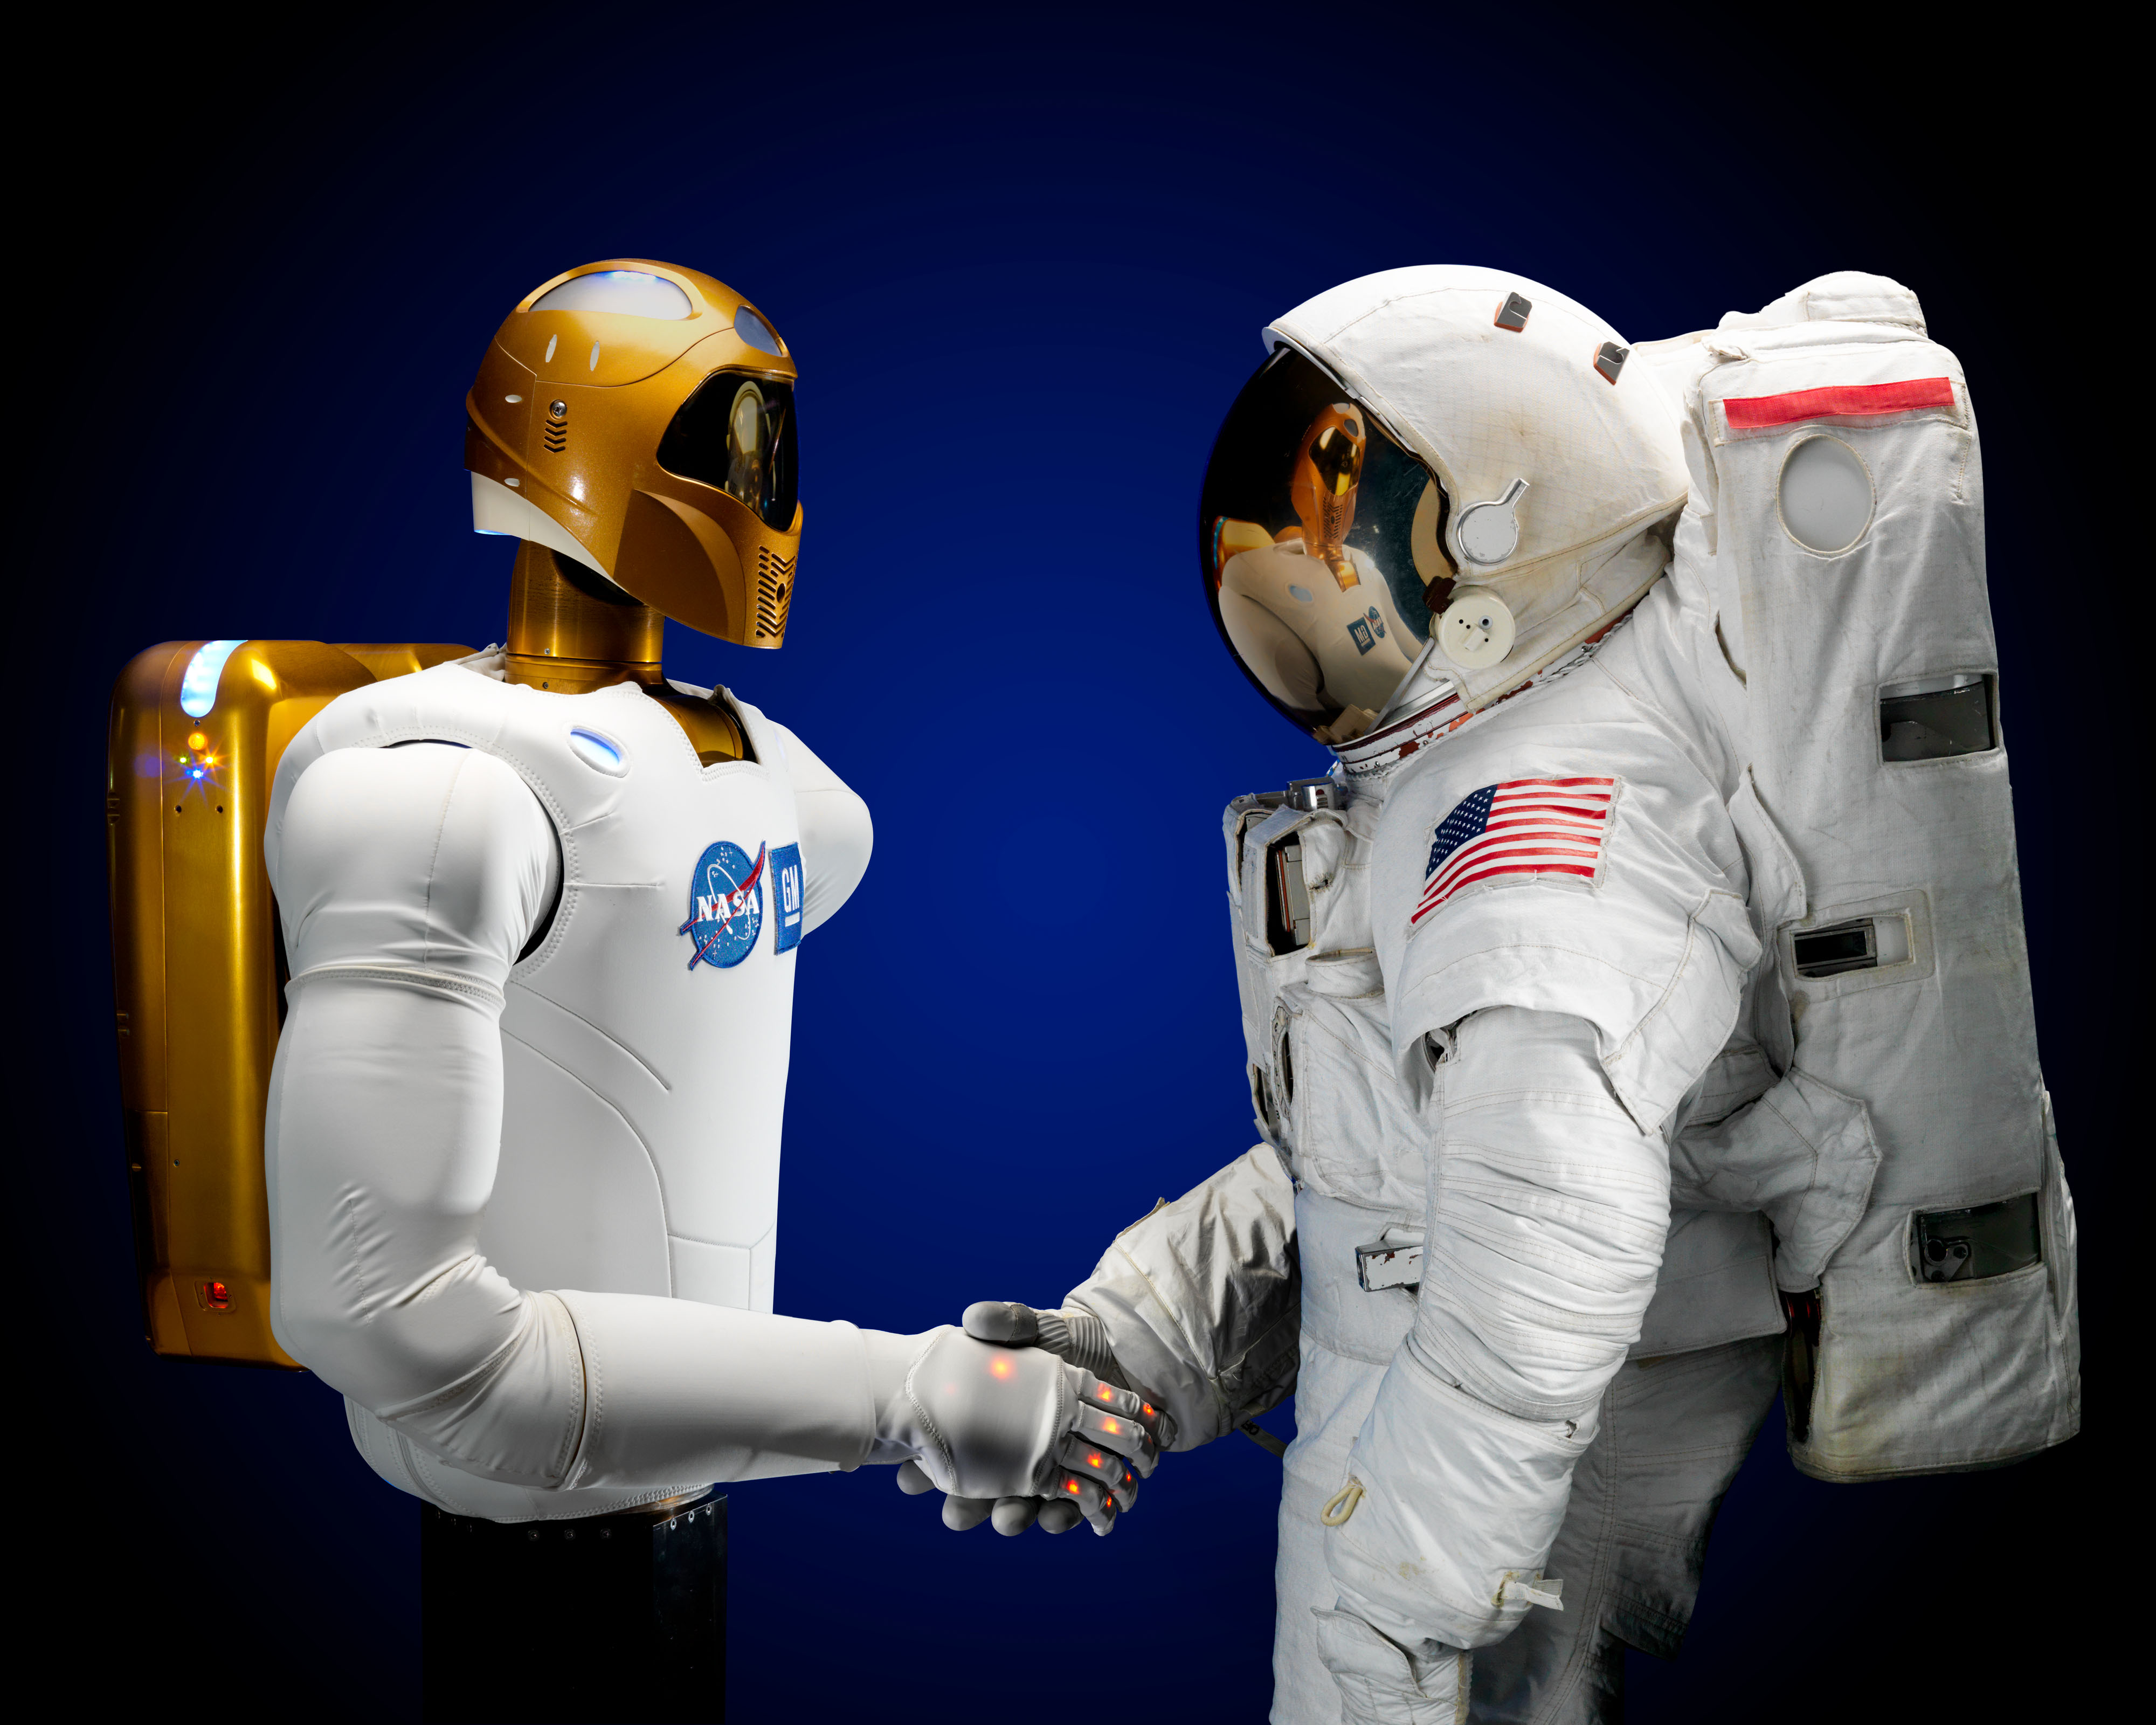
\includegraphics[scale=0.2]{./EtapaModerna/Imagenes/robonaut.jpg}
	\caption{Robonaut (\href{https://www.nasa.gov/images/content/491272main_robonaut2_lg.jpg}{NASA}) (\href{https://pmm.nasa.gov/image-use-policy}{Términos de uso})}
	\label{fig:robonaut}
\end{figure}

En este mismo sentido la compañía canadiense MDA, en su aportación a la ISS, diseñó el robot Dextre con una funcionalidad muy parecida a la ideada para Robonaut. El robot consiste de un cuerpo de enormes dimensiones con dos brazos robóticos capaces de moverse muy rápido. El objetivo de este robot es que sea capaz de realizar tareas para las que antes se requería la salida de alguno de los astronautas de la ISS al exterior de la misma. Este hecho se ha conseguido de tal forma que ni siquiera se tiene por qué operar desde la ISS, si no que se puede realizar el manejo del mismo desde la Tierra. De esta forma, tal y como ocurrió en su primera misión, se pueden realizar tareas de mantenimiento sin necesidad de que los miembros de la ISS estén disponibles o incluso aunque estos estén dormidos. El robot tiene un cuerpo que mide unos 3.5 metros de longitud y dos brazos de 3.5 metros cada uno pesando en total más de 1600 kilogramos.

\begin{figure}[!h]
	\centering
	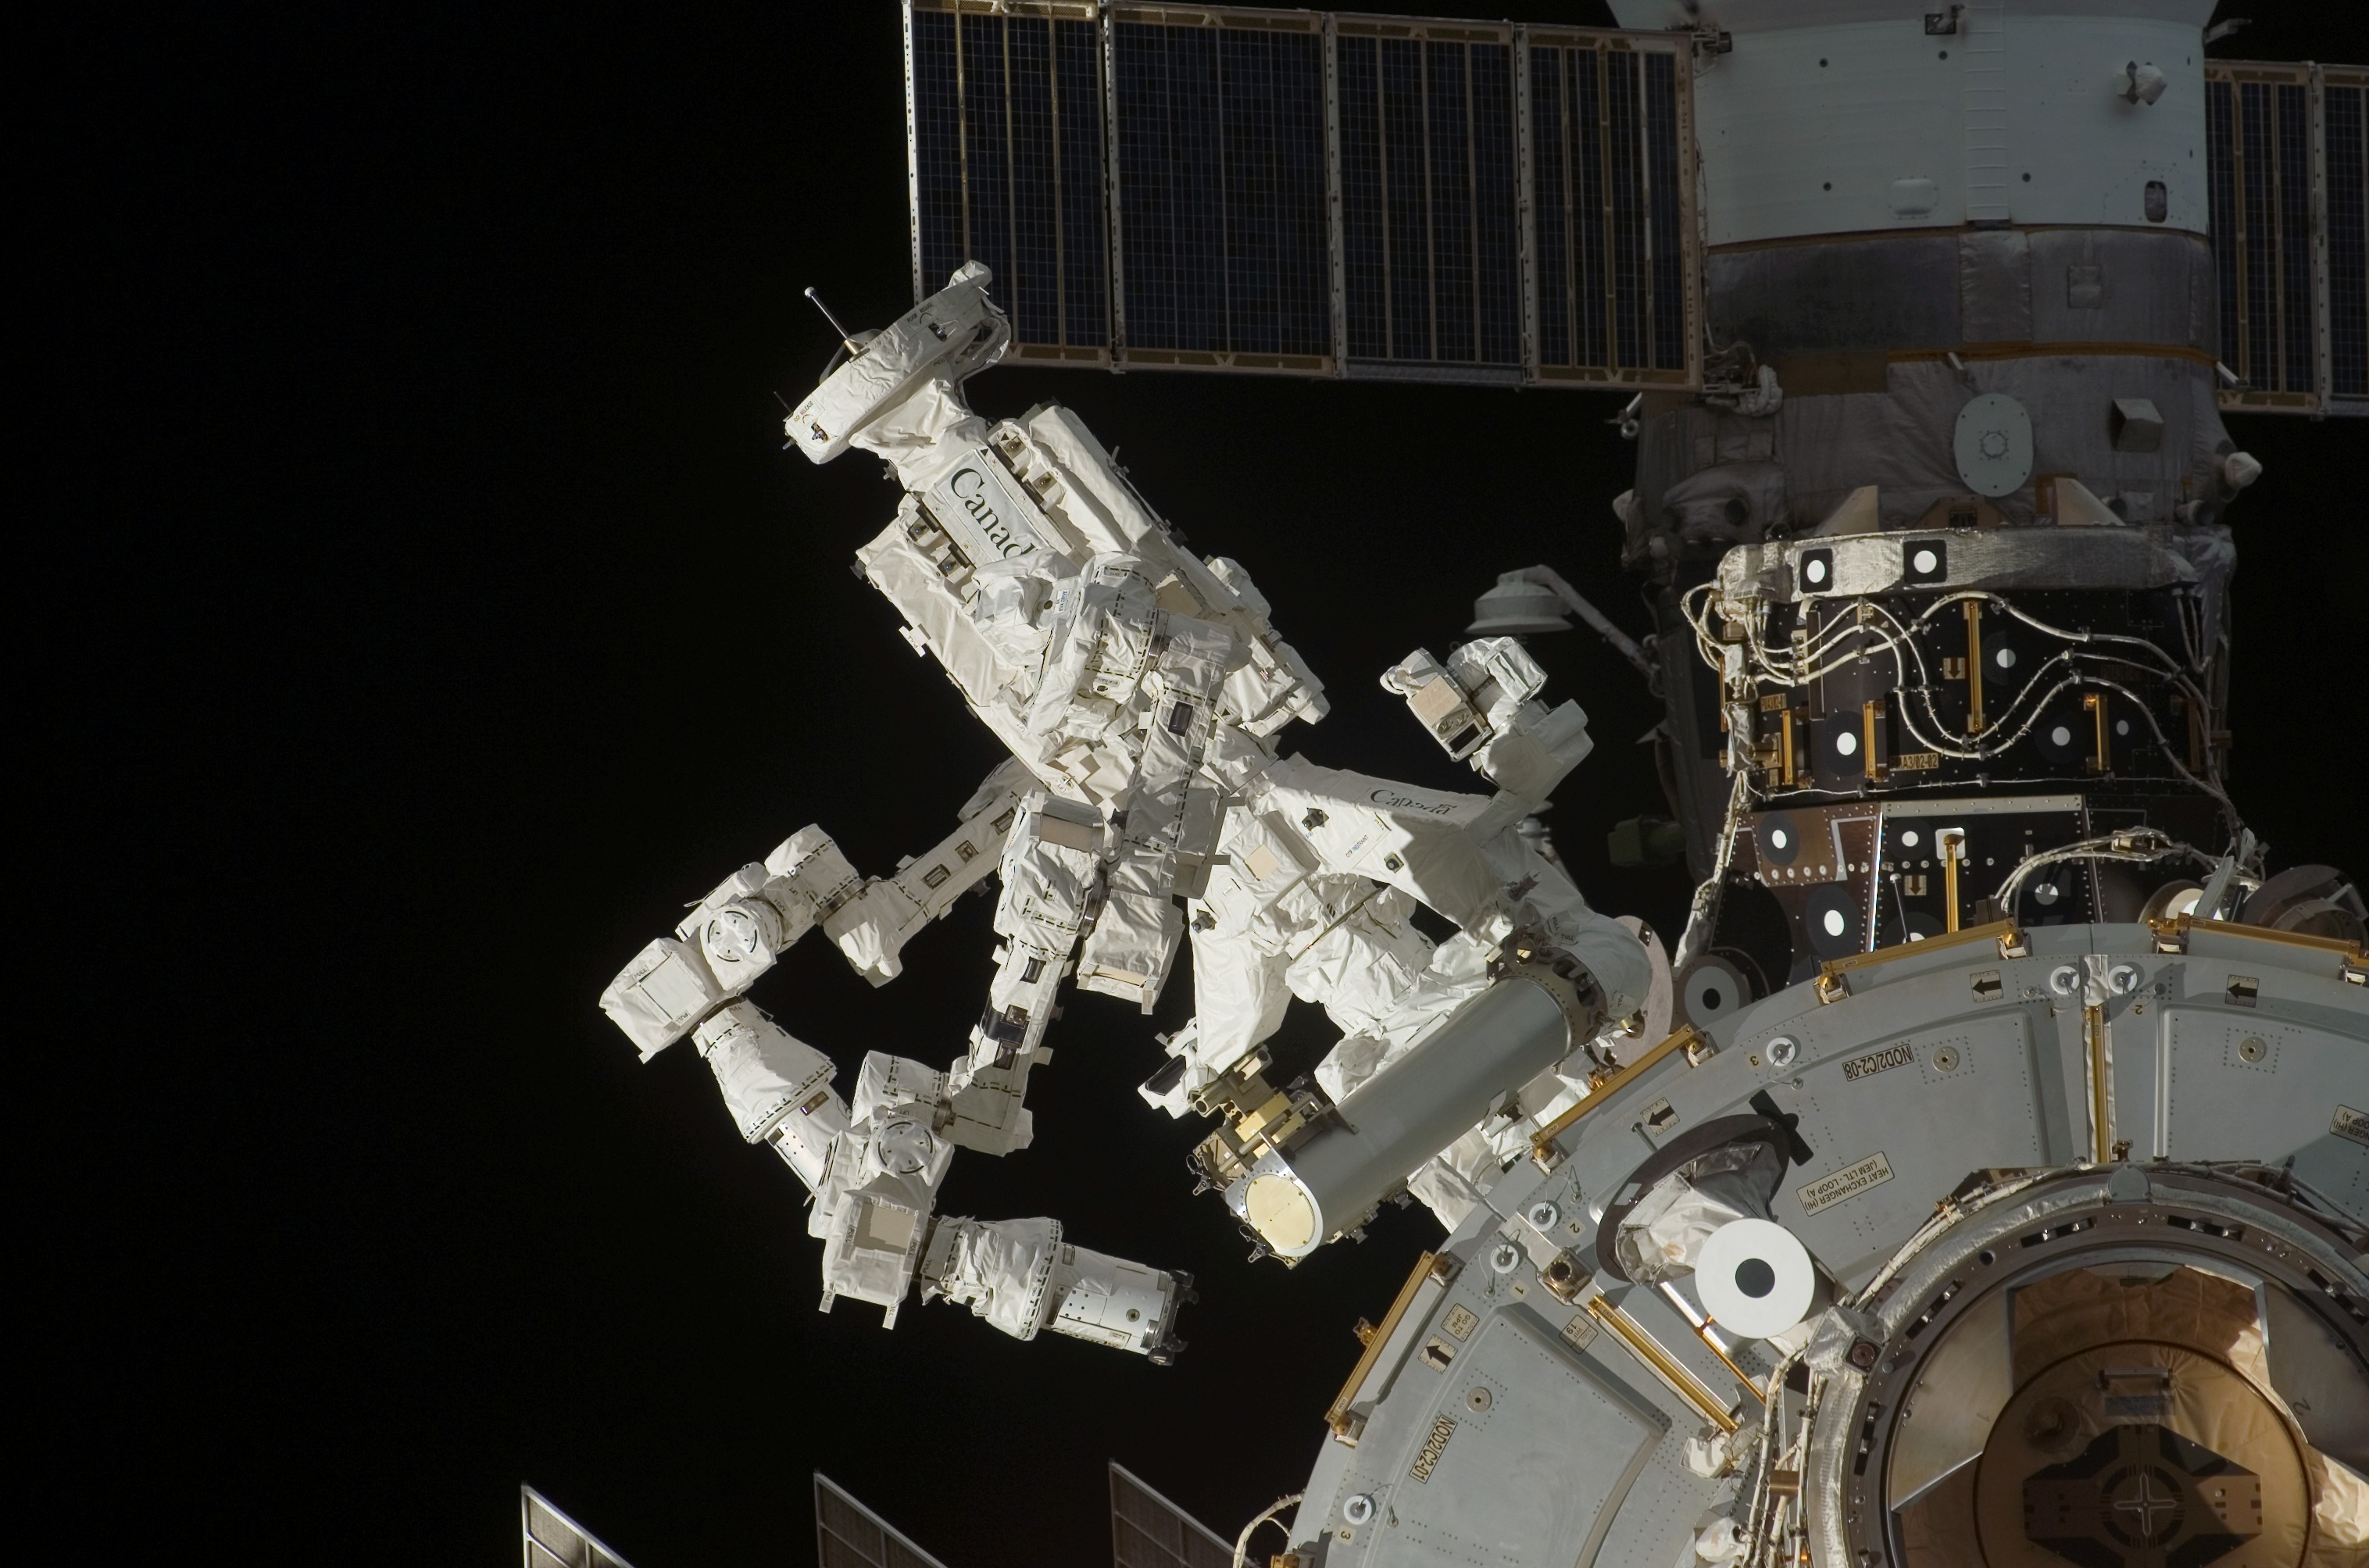
\includegraphics[scale=0.1]{./EtapaModerna/Imagenes/dextre.jpg}
	\caption{Dextre (\href{https://lv.wikipedia.org/wiki/Att\%C4\%93ls:Dextre_on_ISS.jpg}{Wikipedia})}
	\label{fig:dextre}
\end{figure}

La NASA también tiene robots que aún no han sido empleados en misiones reales pero sí se sigue avanzando en su desarrollo, como es el caso del RASSOR (Regolith Advanced Surface Systems Operations Robot). Este robot está diseñado para operaciones de construcción y alisamiento del terreno, extracción de agua, eliminar el hielo de una zona concreta, retirar arena, etc. El RASSOR actualmente está en fase de pruebas, pero se le espera un buen futuro por su mínimo coste de producción y por la versatilidad del mismo, puesto que sería capaz de trabajar unas 16 horas por día durante muchos años. El robot además, por su diseño, está pensado para superar los obstáculos que se le presenten y para poder corregir su posición incluso si vuelca. Para las tareas que se planean que pueda realizar el robot incorpora dos ruedas como las de una trituradora industrial (una en la parte delantera y otra en la trasera) capaces de ser movidas de forma independiente.

\begin{figure}[!h]
	\centering
	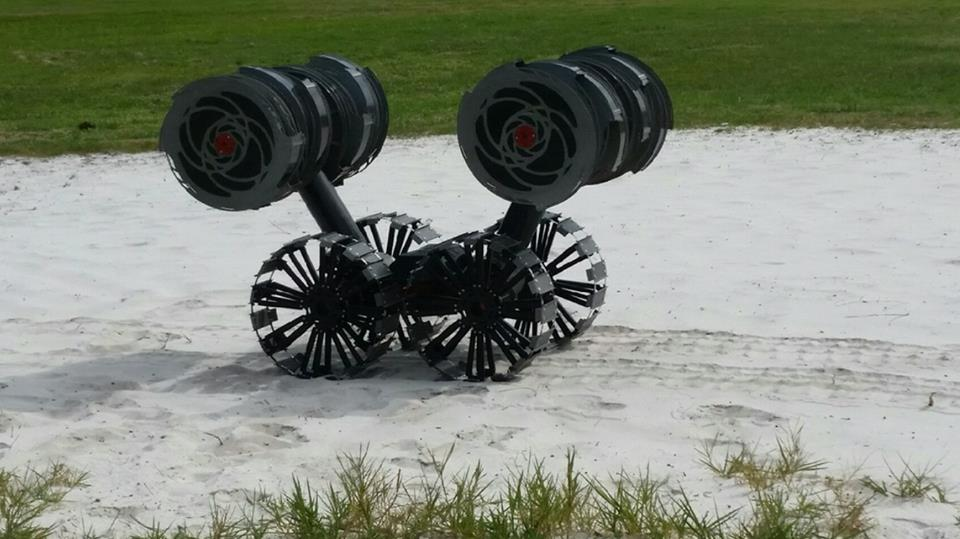
\includegraphics[scale=0.3]{./EtapaModerna/Imagenes/rassor.jpg}
	\caption{RASSOR (\href{https://commons.wikimedia.org/wiki/File:NASA\%27s_Regolith_Advanced_Surface_Systems_Operations_Robot_(RASSOR).jpg}{Wikimedia})}
	\label{fig:rassor}
\end{figure}

En último lugar en los robots creados por la NASA tenemos el que actualmente es la punta de lanza de la compañía: el Curiosity. Este modelo es un vehículo terrestre con componentes robóticos que aglomera todos los conocimientos obtenidos por la NASA en cuanto a robótica. Este robot pertenece a la serie de los Rovers y actualmente está cumpliendo su misión de exploración de la superficie marciana. El Curiosity fue lanzado hacia Marte en el año 2011 y aterrizó en el año 2012 tras un viaje de unos 8 meses. El robot tiene un complejo sistema de análisis que permite que opere de forma autónoma, ya que en este caso la distancia del operador (la Tierra) y el vehículo es tan grande que llevaría unos 14 minutos mandar una orden desde las oficinas de la NASA y que el Curiosity la recibiera. El robot pesa unos 900 kilogramos, midiendo 2.9 metros de largo, 2.7 metros de ancho y 2.2 metros en altura. En cuanto a capacidad de computación se incorporan chips de IBM diseñados específicamente para el mismo, ya que al estar en Marte y haber tenido que soportar el viaje por el espacio se requiere que todos los dispositivos tales como microprocesadores, memoria RAM y memoria flash vayan convenientemente aisladas de la radiación, pues podrían verse alterados los datos o incluso dejar de funcionar. Para alimentar los sistemas eléctricos, el Curiosity incorpora un generador de energía por radioisótopos con lo que lleva incluido 4.8 kilogramos de dióxido de plutonio 238 que le dan una autonomía mínima de 14 años desde su despliegue. En cuanto a el equipo robótico el Curiosity incorpora un sistema de suspensiones y ruedas pensadas para poder superar fácilmente los obstáculos del terreno marciano tales como roca o arena. Todo el sistema de movilidad del robot está diseñado para que, mediante un sistema complejo de cámaras llamadas Hazcams (Hazard Cameras) se detecte el terreno del Rover en un entorno circular de 3 metros a su alrededor de forma que sea capaz de predecir si un obstáculo será o no superable para él. La velocidad del vehículo no es nada elevada siendo su velocidad media 30 metros por hora, pudiendo llegar al pico de 90 metros por hora.

\vspace{10px}

En cuanto al equipamiento técnico para obtener datos de Marte el Curiosity incorpora los siguientes elementos:

\begin{enumerate}
  \item MastCam (Mast Camera): está compuesta por dos cámaras independientes capaces de sacar fotos true-color y vídeo a 10 fotogramas por segundo. Cada cámara incorpora una memoria de 8 GB capaces de almacenar 5500 imágenes sin compresión.
  \item ChemCam (Chemistry and Camera complex): este sistema de cámaras incorpora un sistema de análisis por rayos X, espectrómetros y cámaras que analizan muestras del suelo marciano para obtener su composición.
  \item SAM (Sample Analysis at Mars): el objetivo de este módulo es analizar compuestos orgánicos y gases tanto de la atmósfera como de muestras sólidas. Incorpora un espectrómetro de masas, un cromatógrafo de gases y un espectrómetro láser.
  \item DRT (Dust Removal Tool): esta herramienta sirve al robot para limpiar el polvo de las rocas o terreno sobre el que se quiere obtener una muestra.
  \item RAD (Radiation assessent detector): esta herramienta fue diseñada para medir la radiación a la que se expone una nave en un viaje interplanetario con la intención de saber qué requisitos deben tener las naves espaciales para poder llevar personas en distancias tan largas. Además, actualmente, este módulo se está usando para saber los niveles de la radiación en el propio planeta.
  \item DAN (Dynamic Albedo of Neutrons): este tubo de neutrones se utiliza para poder obtener medidas de hidrógeno, agua o hielo en la superficie de Marte.
  \item MARDI (Mars Descent Imager): la función que cumplió este módulo fue tomar un buen número de imágenes durante el aterrizaje para poder hacer un mapeado del terreno alrededor del Curiosity, de forma que se tuviera una información de qué terreno rodeaba al robot y localizar su posición de aterrizaje.
  \item Brazo robótico: el Curiosity incorpora un único brazo robótico de 2.1 metros de largo y 30 kilogramos de peso. El brazo sirve al robot para poder tomar las muestras y mover elementos como por ejemplo pinzas para tomar muestras, un taladro de pequeñas dimensiones para tomar muestras sólidas, el DRT, etc.
\end{enumerate}

\begin{figure}[!h]
	\centering
	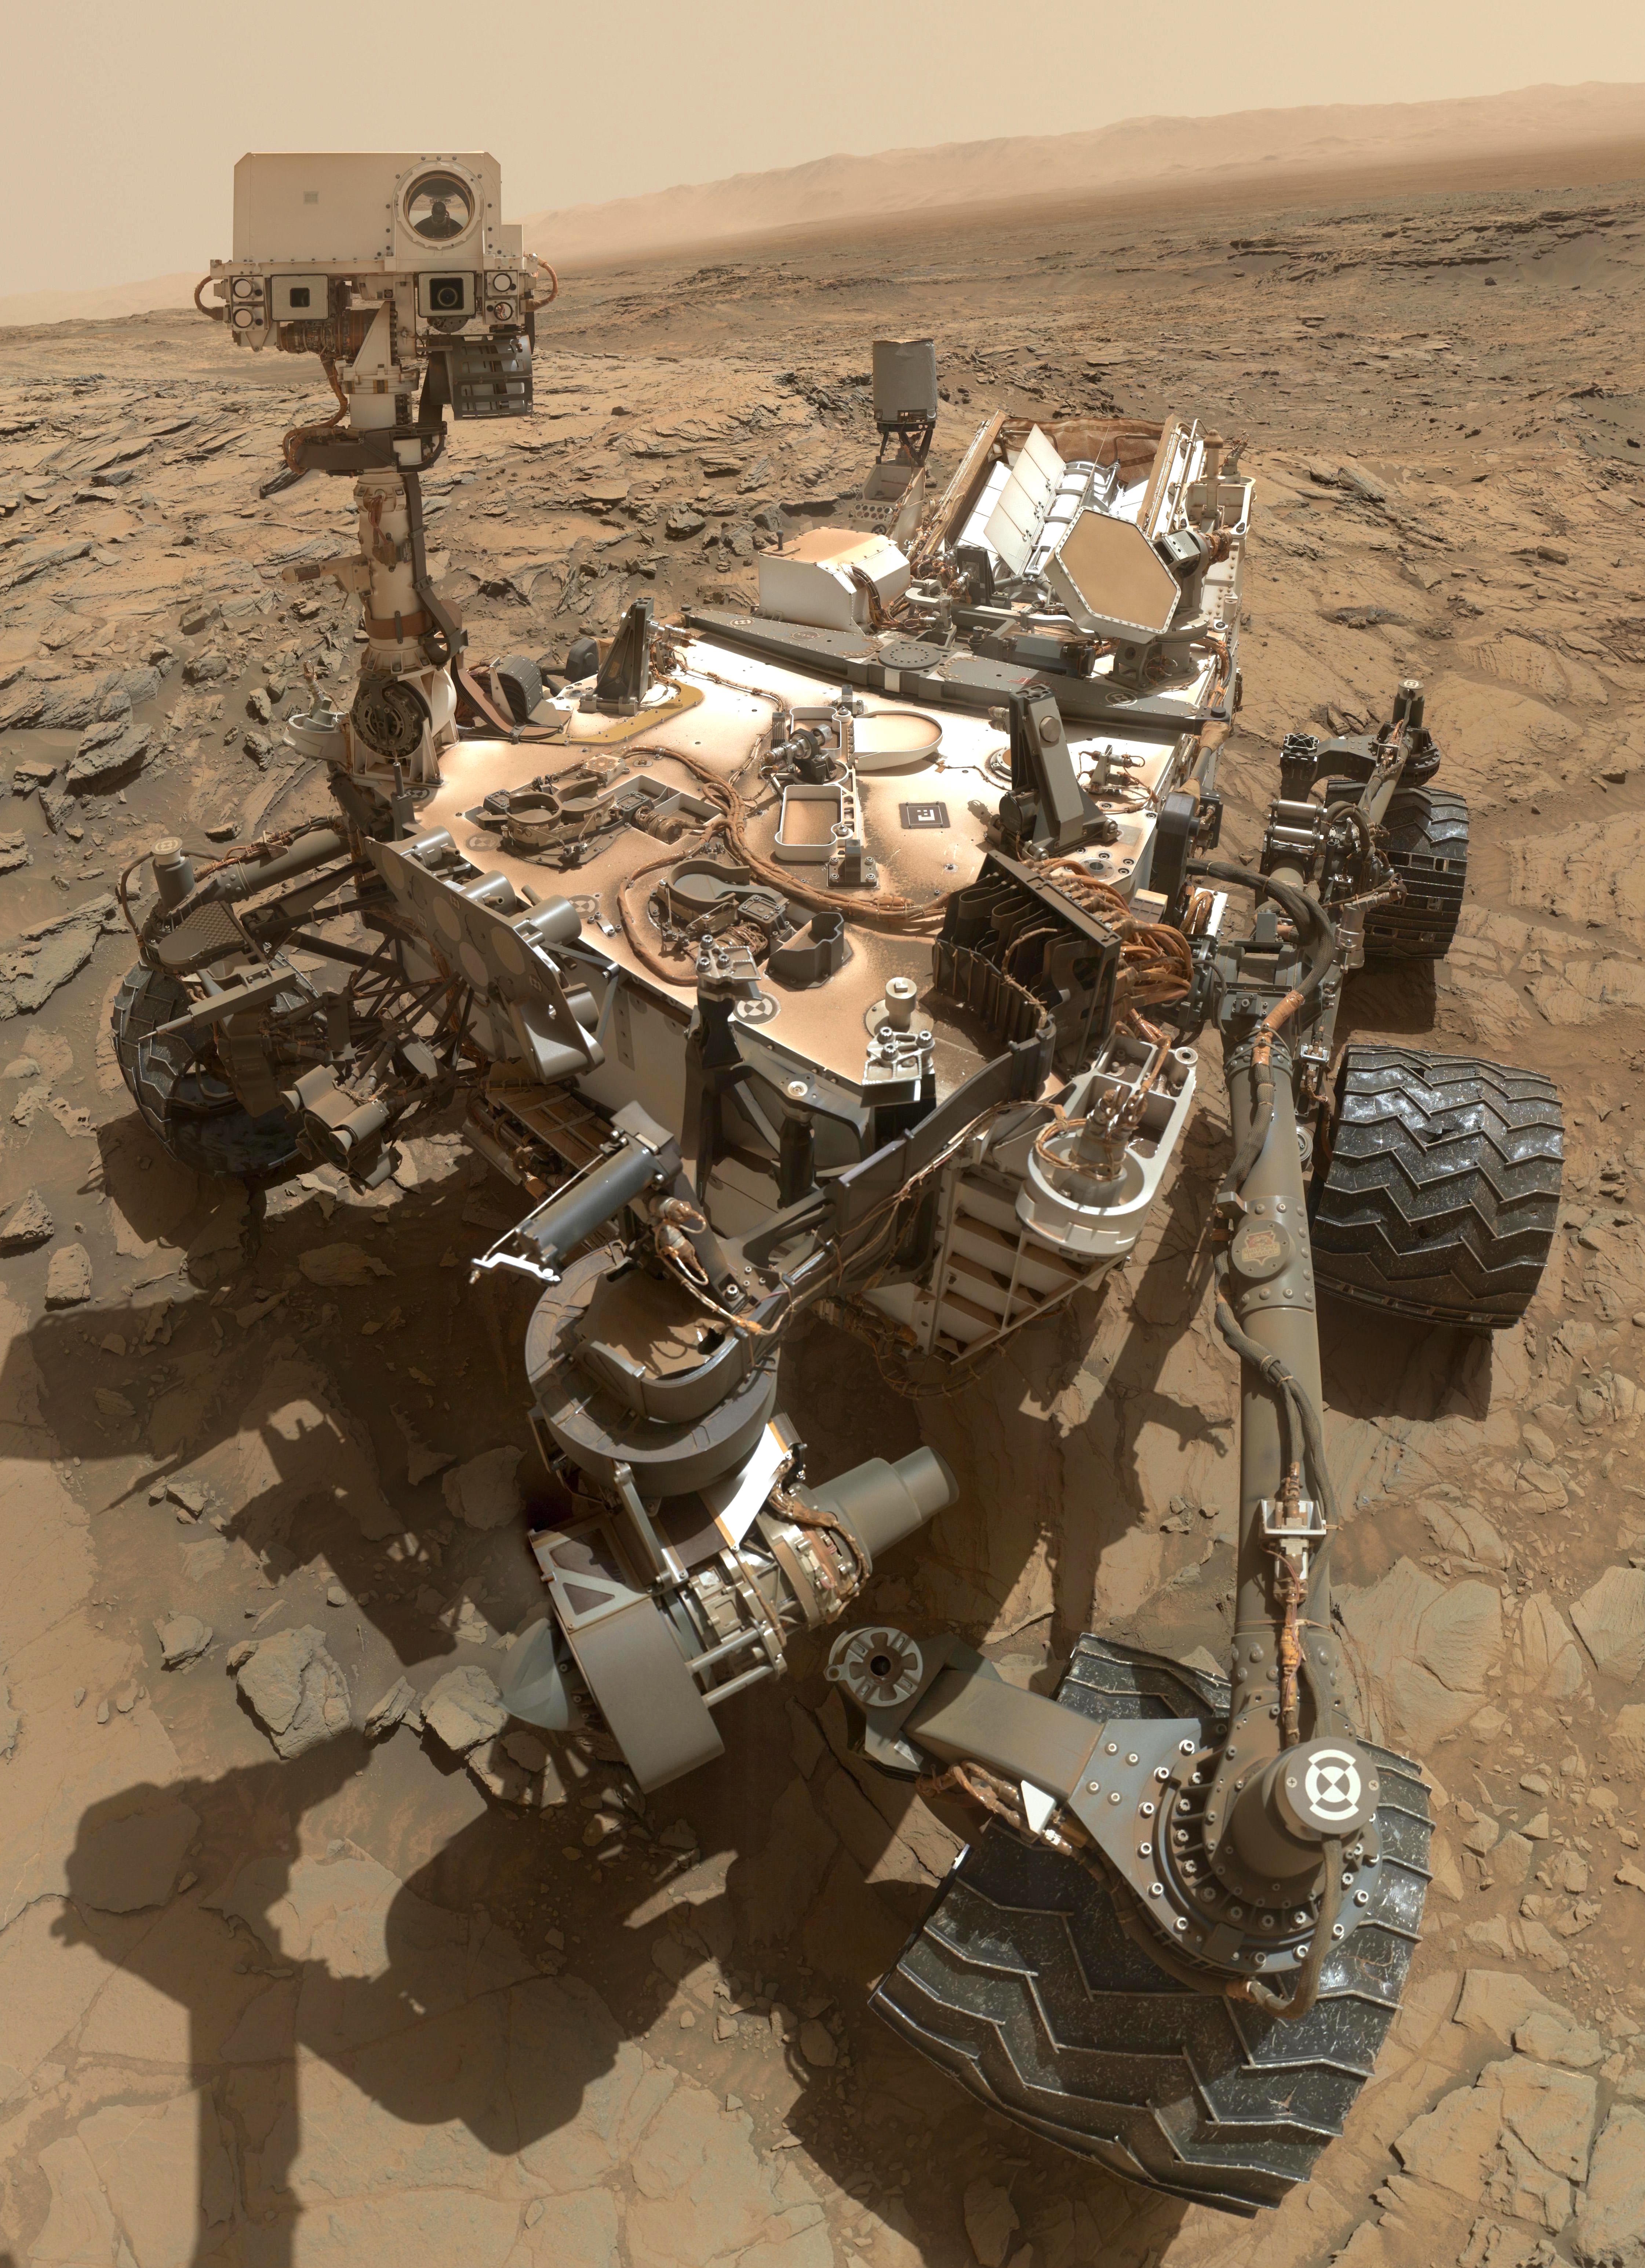
\includegraphics[scale=0.035]{./EtapaModerna/Imagenes/curiosity.jpg}
	\caption{Curiosity (\href{https://en.wikipedia.org/wiki/File:Curiosity_Self-Portrait_at_\%27Big_Sky\%27_Drilling_Site.jpg}{Wikimedia})}
	\label{fig:curiosity}
\end{figure}

Estos avances han sido cruciales en el desarrollo de la ciencia y la tecnología tanto por las altas inversiones de dinero que fomentan la investigación como por los experimentos realizados gracias a la tecnología desarrollada por la NASA. Actualmente se siguen liderando propuestas innovadoras tales como Mars 2020 o el reciente proyecto (ya aterrizado en Marte) Mars InSight.

\subsubsection{Robots militares}
En el ámbito de la industria militar y el equipo empleado en la guerra se ha realizado un avance enorme en el tipo de tecnología que se involucra en la robótica. En esta área no se persiguen interfaces conversacionales complejas ni robots con forma humana (por el momento) si no que está más enfocada en vehículos no tripulados que se manejen por sí solos o teleoperados de forma que la guerra, en su gran mayoría no sea un combate cuerpo a cuerpo para minimizar las pérdidas humanas desde el lado del atacante. En este sentido la robótica comenzó a tomar parte desde la Segunda Guerra Mundial y la posterior Guerra Fría, época en la que la inversión en el material militar aumentó considerablemente tanto en Europa en general como en Estados Unidos y Rusia en particular, por lo que estos países jugarán una baza importante en el desarrollo de la tecnología al ser los implicados directamente en los conflictos bélicos.

\vspace{10px}

Actualmente hay muchos robots en desarrollo que serán importantes en un futuro en las misiones a las que se los destine, pero podemos destacar desde un punto de vista de la relevancia y actualidad de los mismos a los siguientes modelos:

\begin{enumerate}
  \item Daksh de DRDO: este robot no está pensado para el uso directo en el combate atacando objetivos, si no que se ideó con el propósito de que fuese capaz de inutilizar material explosivo antes de que las tropas pasaran por un lugar concreto. El robot funciona mediante baterías y es capaz de operar por él solo levantando objetos y remolcando vehículos para despejar el camino. Además incorpora un mecanismo de desactivación de bombas que consiste en inyectar agua a alta presión para inutilizar el material. Todas estas labores las puede hacer el robot por sí mismo, por lo que está diseñado para analizar el terreno a su alrededor, ser capaz de esquivar o superar obstáculos y organizar las tareas que debe llevar a cabo para desactivar bombas. A pesar de todo esto, si el equipo de combate necesita operarlo manualmente, incorpora un sistema de comunicación que permite su operación remota.
  \begin{figure}[!h]
  	\centering
  	\includegraphics[scale=0.2]{./EtapaModerna/Imagenes/daksh.JPG}
  	\caption{Daksh (\href{https://commons.wikimedia.org/wiki/File:Daksh_-_Remotely_Operated_Vehicle_-_DRDO_-_Pride_of_India_-_Exhibition_-_100th_Indian_Science_Congress_-_Kolkata_2013-01-03_2570.JPG}{Wikimedia})}
  	\label{fig:daksh}
  \end{figure}
  \newpage
  \item Elbit Hermes 450: este vehículo aéreo entra dentro de la categoría de los llamados UAV (Unmanned Aerial Vehicle). El objetivo de este vehículo es la exploración del terreno y detección de posibles objetivos y peligros. Actualmente muchos países han adquirido este UAV que es capaz de operar durante 17 horas seguidas. El robot tiene un alto grado de independencia de los operadores, puesto que se puede pedir que explore una zona concreta y él lo hará todo autónomamente, aún así también se incorpora un sistema de comunicación por satélite para operarlo manualmente si se requiere. Aunque en un principio se diseñó como vehículo exploratorio, actualmente hay algunos países como Estados Unidos que han incorporado misiles a este UAV, de forma que también se podría emplear en el derribo de objetivos. Dentro de esta misma categoría podríamos meter a los MQ-9 de Estados Unidos cuya misión es la misma que la que cumple el Elbit Hermes 450.
  \begin{figure}[!h]
  	\centering
  	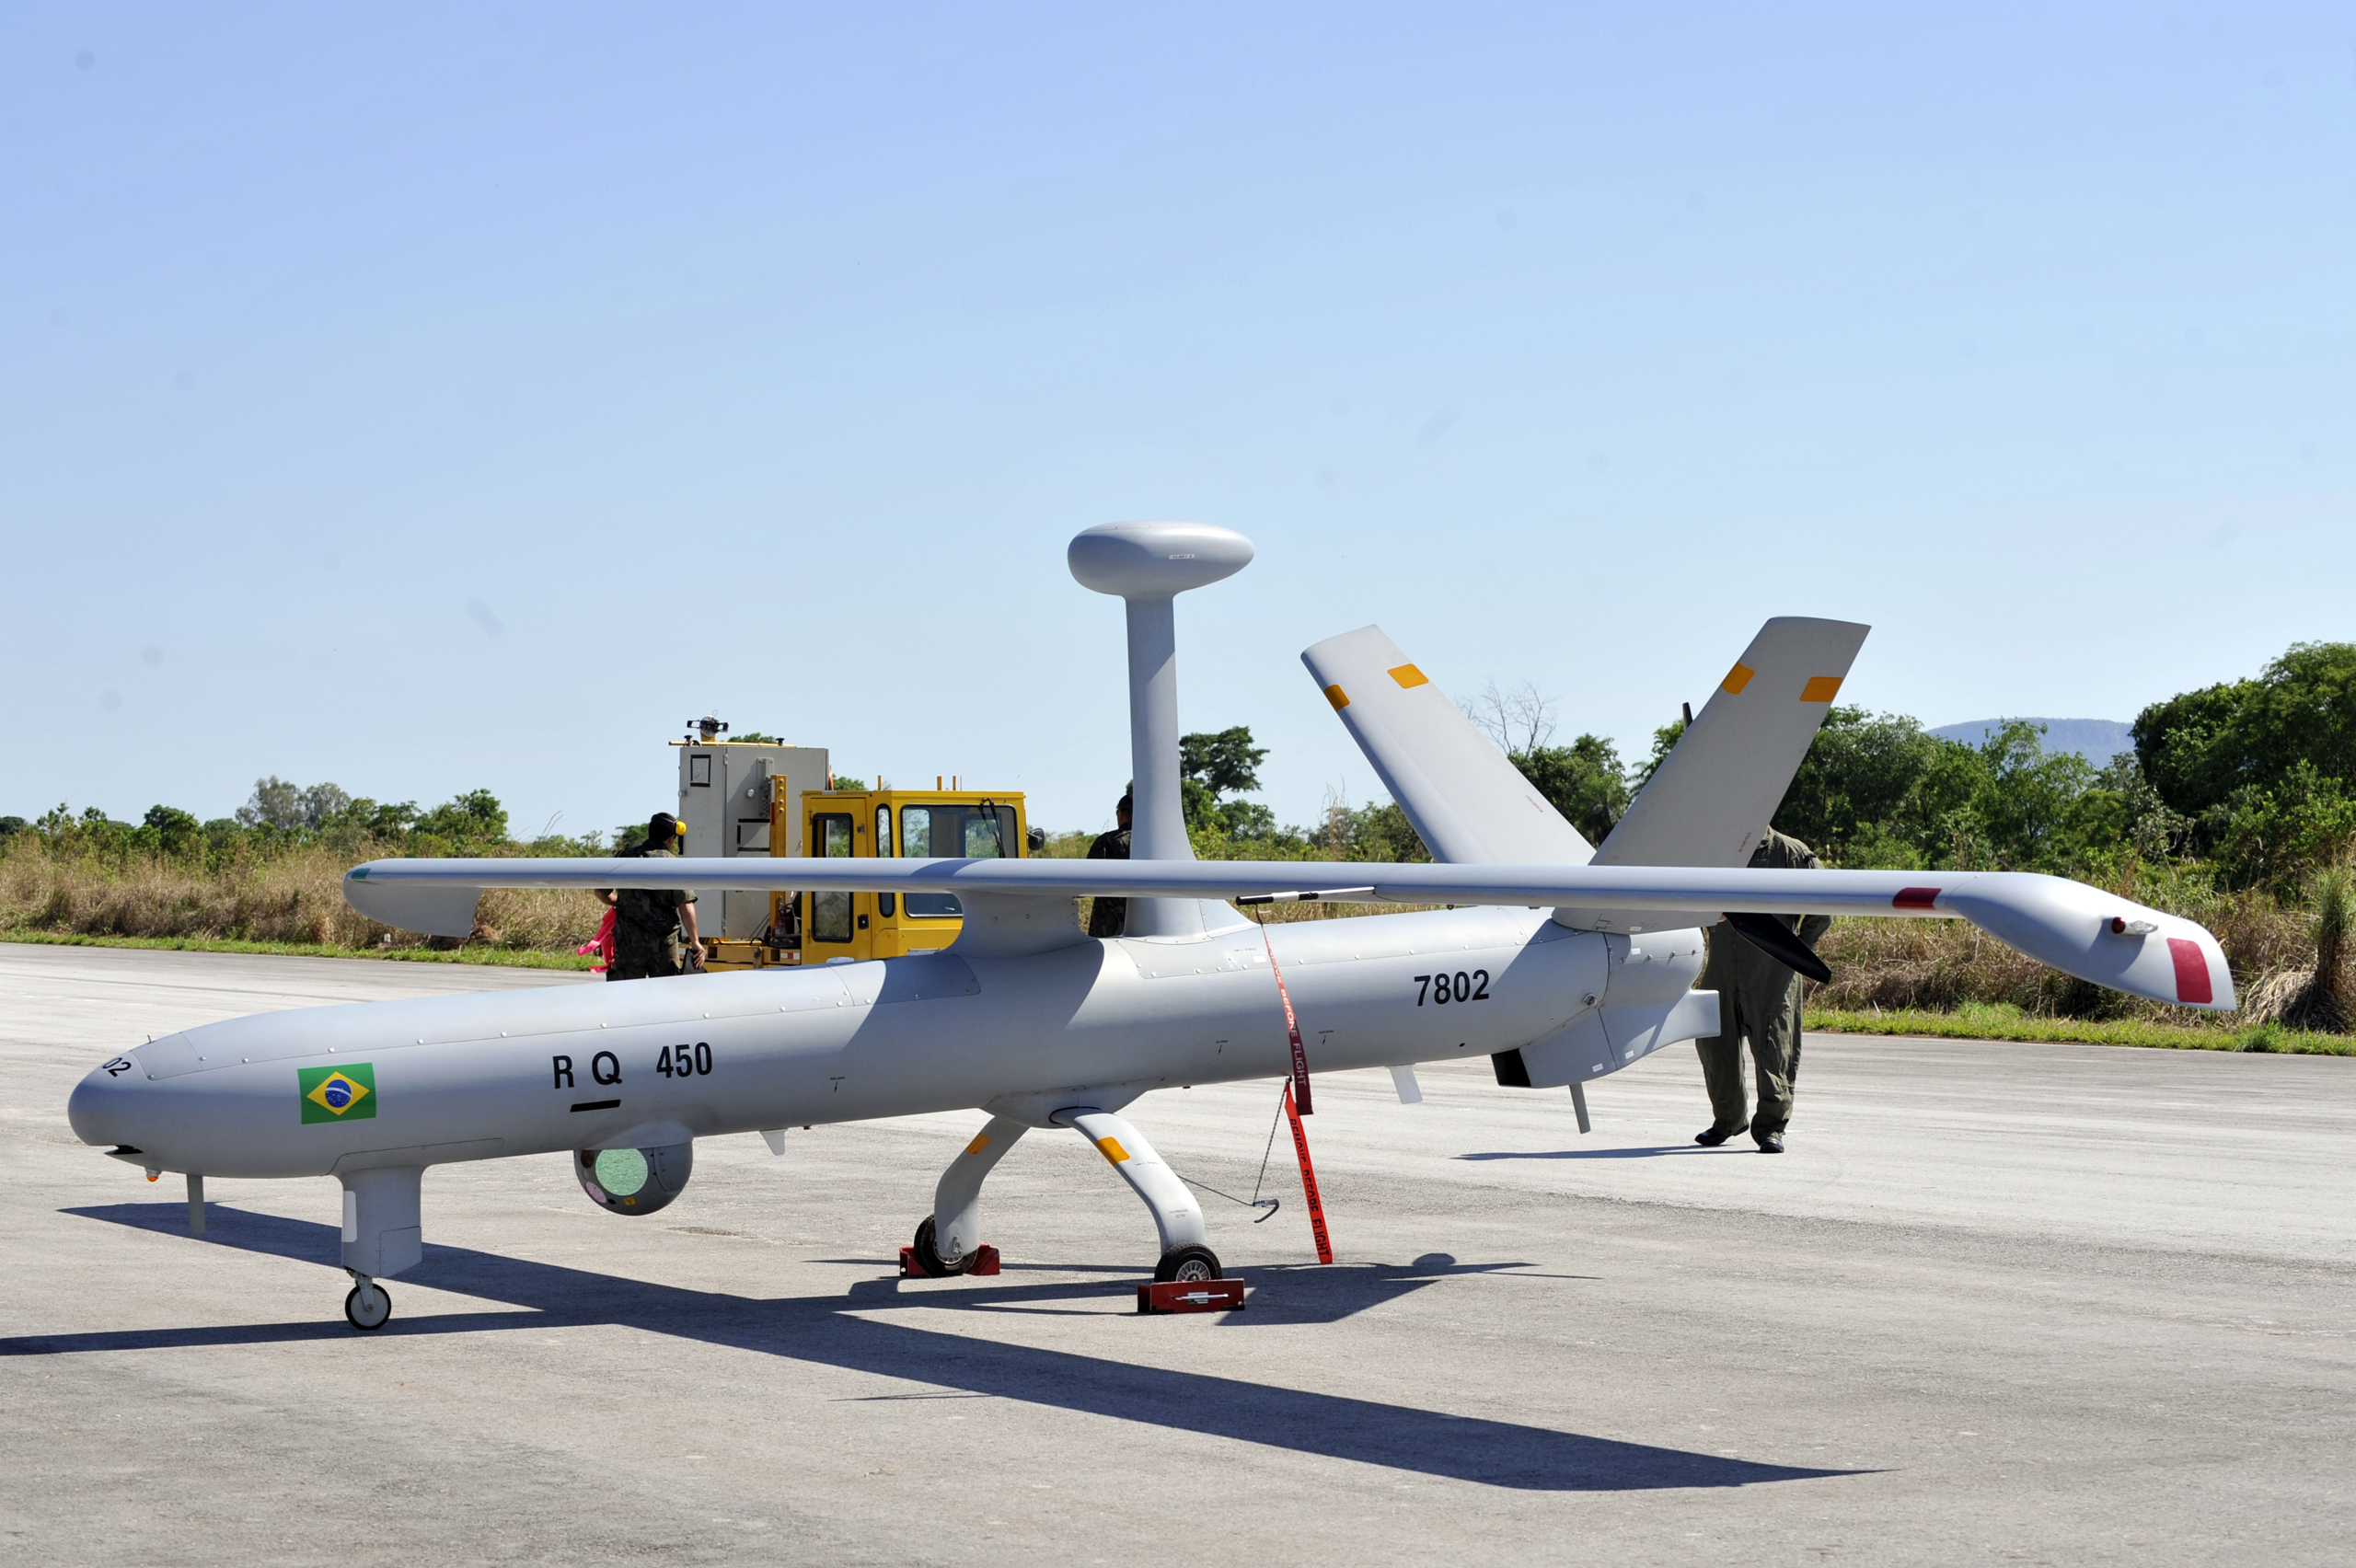
\includegraphics[scale=0.3]{./EtapaModerna/Imagenes/elbit_hermes_450.jpg}
  	\caption{Elbit Hermes 450 (\href{https://commons.wikimedia.org/wiki/File:Vant_Hermes_450_da_FAB_no_aeroporto_de_C\%C3\%A1ceres_(MT)_(8101398607).jpg}{Wikimedia})}
  	\label{fig:elbithermes450}
  \end{figure}
  \item Goalkeeper CIWS (Close-in Weapon System): el Goalkeeper es un sistema autónomo de defensa de embarcaciones de corto alcance. El sistema incorpora una metralleta GAU-8 de calibre 30 capaz de, mediante un sistema de reconocimiento de objetivos, fijar la mayor amenaza que tiene el barco y comenzar el ataque hacia la misma. Este propósito es resuelto mediante dos radares con los que se pueden obtener los objetivos a atacar, calcular la distancia y posición de los mismos y poder detectar el que él considera mas amenazador. Además el sistema es capaz de detectar la velocidad a la que viaja el enemigo y predecir la trayectoria, cosa que es imprescindible para poder acertar en el blanco.
  \begin{figure}[!h]
  	\centering
  	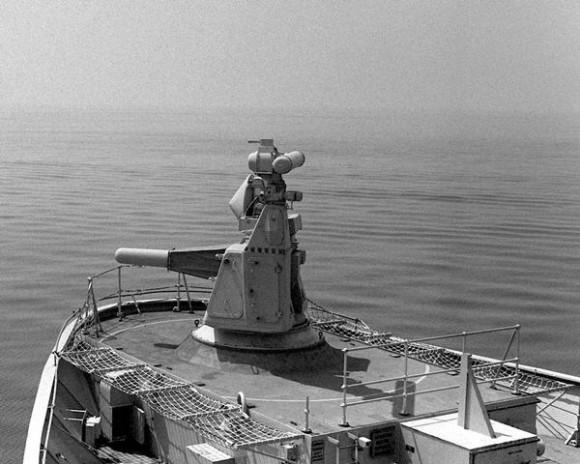
\includegraphics[scale=1.3]{./EtapaModerna/Imagenes/Goalkeeper.jpg}
  	\caption{Goalkeeper (\href{https://commons.wikimedia.org/wiki/File:Goalkeeper.jpg}{Wikimedia})}
  	\label{fig:goalkeeper}
  \end{figure}
  \item Guardium: también se requieren en la industria robots que operen de forma autónoma en el ámbito terrestre en la batalla. Actualmente este modelo ha sido empleado por Israel en la franja de Gaza. El robot puede operar de forma autónoma fijándole objetivos o teleoperado con lo que un militar podría dirigir el robot hacia el objetivo manualmente. El robot va equipado con una armadura externa para resistir los impactos de bala y armamento tanto de supresión del enemigo (no letal) como armamento pesado de guerra. Incorpora cámaras infrarrojas, radares, micrófonos de alta sensibilidad y un conjunto de sensores capaces de detectar de dónde vienen los disparos para poder protegerse. Si el robot entra en modo autónomo analiza sus alrededores y toma decisiones sobre las localizaciones a las que se debe dirigir identificando al enemigo. El robot tiene una autonomía de 103 horas de uso continuado y se suele utilizar en rondas de vigilancia para protección de las personas en zonas de conflicto. Las cámaras no sólo duran las 103 horas comentadas, si no que además incorporan un sistema de emergencia que podrían hacer que las cámaras funcionasen 24 horas extra por si son necesarias en alguna misión de vigilancia.
  \begin{figure}[!h]
  	\centering
  	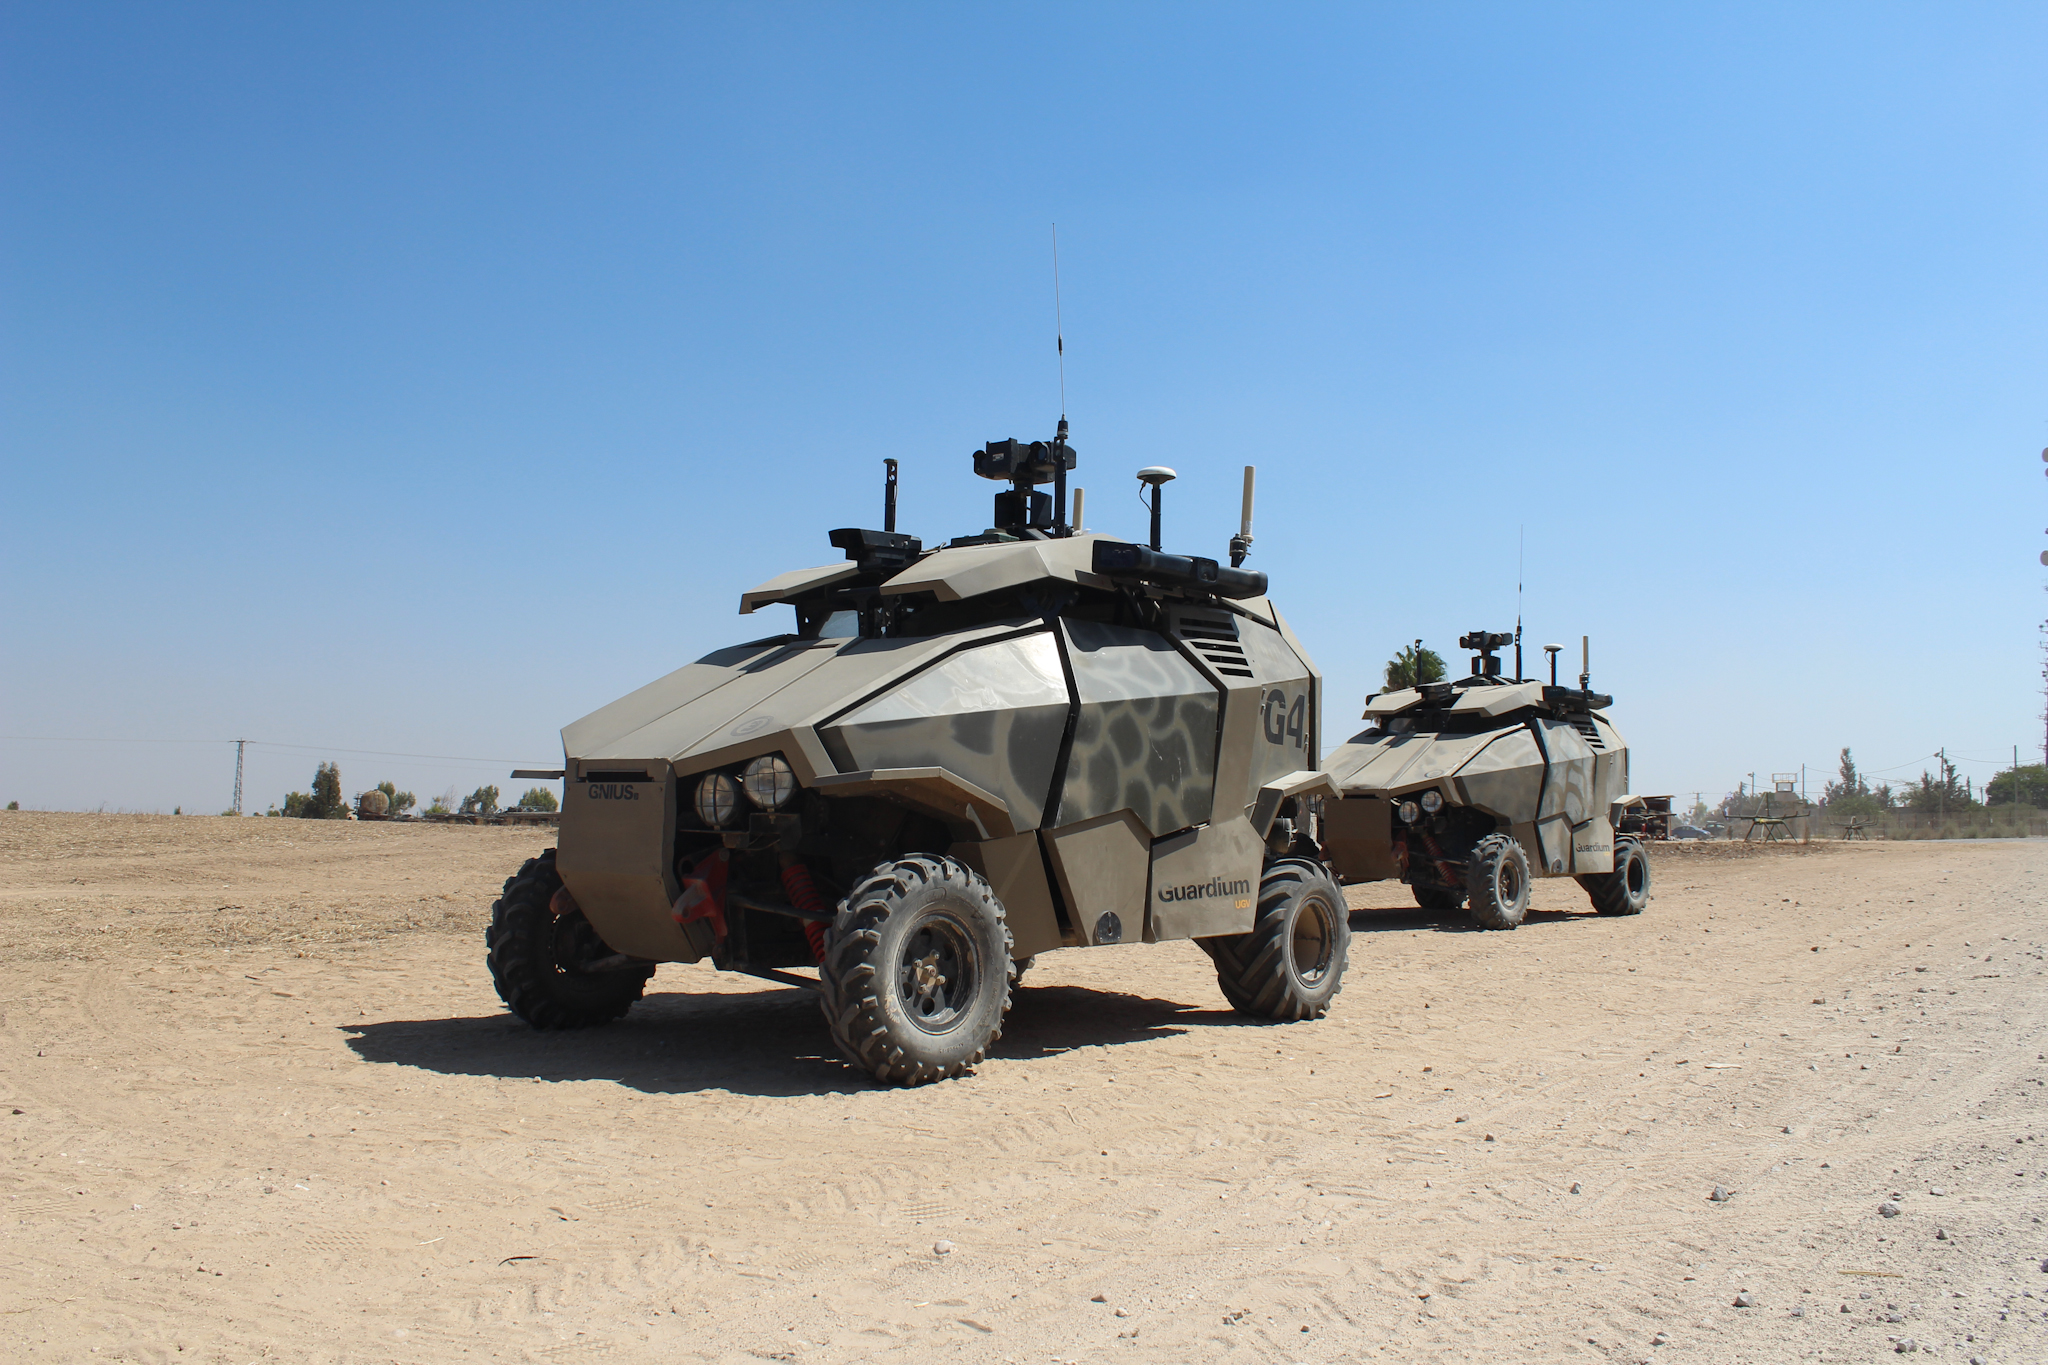
\includegraphics[scale=0.13]{./EtapaModerna/Imagenes/guardium.jpg}
  	\caption{Guardium (\href{https://ca.wikipedia.org/wiki/Fitxer:Flickr_-_Israel_Defense_Forces_-_Israeli_Made_Guardium_UGV_(5).jpg}{Wikipedia})}
  	\label{fig:guardium}
  \end{figure}
  \item TALON: El TALON es un robot terrestre no tripulado usado en la guerra de Bosnia con la intención de reducir las amenazas por explosivos a las tropas que se desplazan de forma terrestre. El robot está diseñado de forma modular, de esta manera cada país puede adaptarlo mediante la incorporación o retirada de sensores del mismo. El robot está pensado para poder desplazar los elementos de su entorno con la intención de despejar el camino e investigarlo. Para ello tiene una capacidad de carga de 45 kilogramos, una capacidad de tomar 77.11 kilogramos con su pinza, remolcar 340 kilogramos y la capacidad de levantar hasta 9 kilogramos con su brazo. El robot incorpora micrófonos para escuchar su entorno y altavoces para que sirva de elemento de comunicación de ser necesario. Adicionalmente TALON puede incorporar sensores de detección de gases, químicos, radiación, temperatura, GPS y brújula. Si se requiere que el mismo tenga una mayor fuerza y capacidad de carga con su brazo se le puede añadir un eje de rotación mejor que ayudaría a llevar por ejemplo armas de largo alcance. En el terreno de la desactivación de explosivos también pueden incorporarse al mismo sensores de rayos X, una escopeta, herramientas de corte de cables, etc. El robot es operado mediante un portátil y joysticks que controlan tanto el movimiento como el brazo y los elementos añadidos al mismo. Para ello el robot incorpora baterías recargables y un paquete de baterías extra no recargables para casos de emergencia. Además la comunicación se realiza mediante un sistema de cámaras rotatorias, cámaras térmicas y micrófonos de forma que el operador tenga una información muy detallada de lo que rodea al TALON.
  \begin{figure}[!h]
  	\centering
  	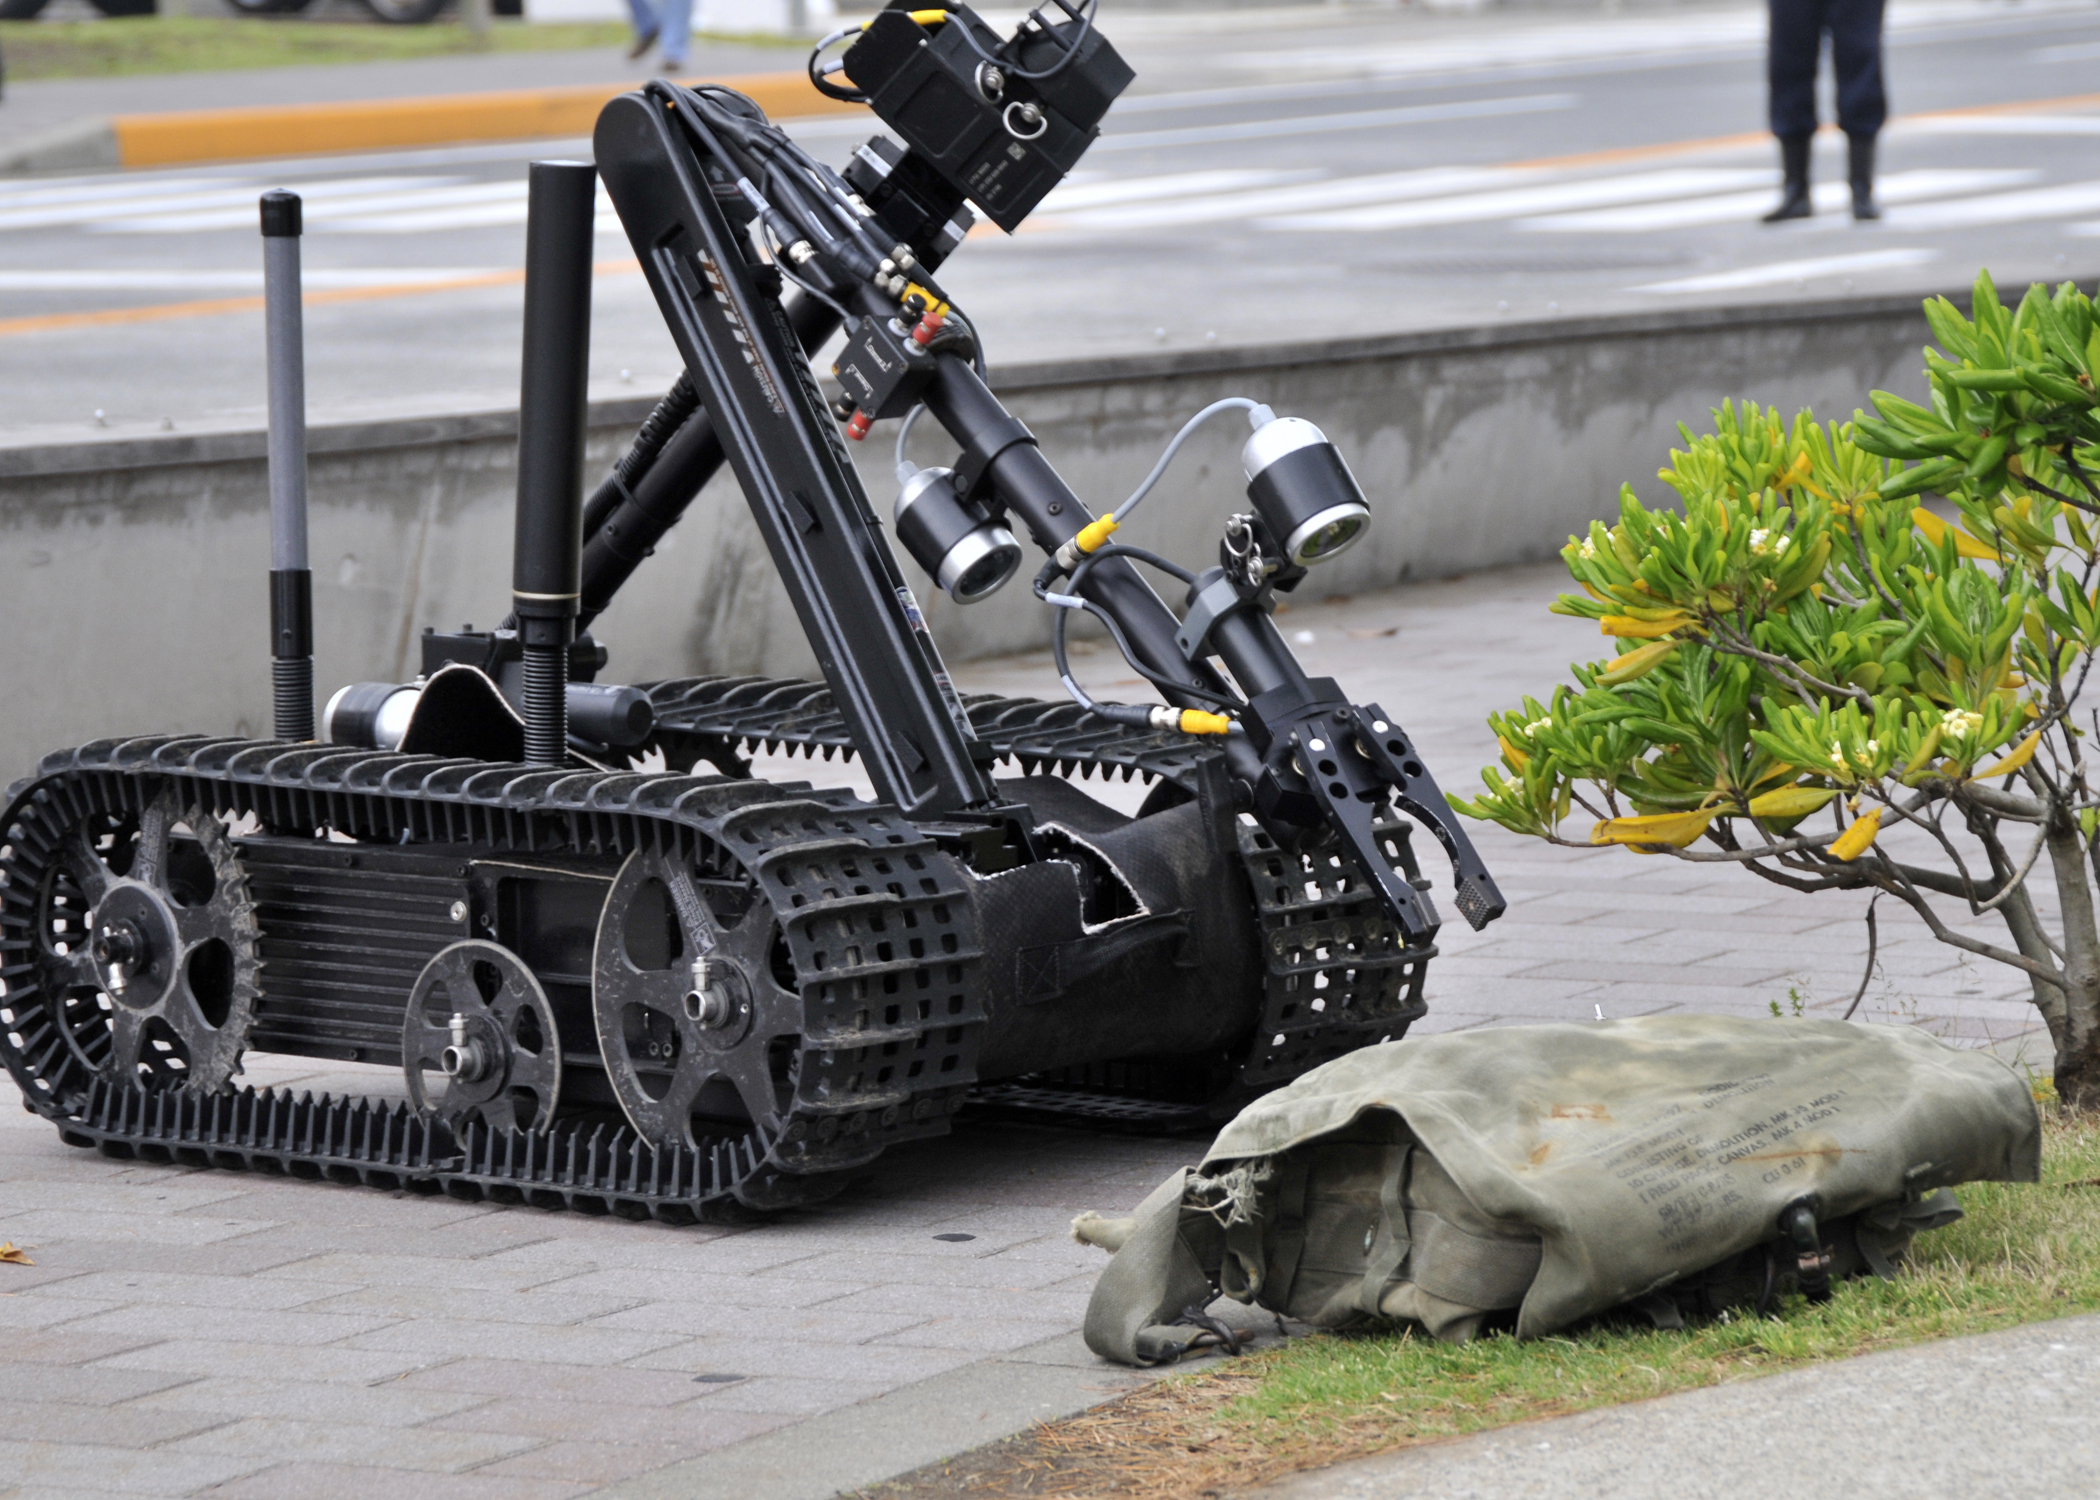
\includegraphics[scale=0.5]{./EtapaModerna/Imagenes/talon.jpg}
  	\caption{TALON (\href{https://commons.wikimedia.org/wiki/File:US_Navy_090512-N-2013O-013_A_Mark_II_Talon_robot_from_Explosive_Ordnance_Disposal_Mobile_Unit_5,_Det._Japan,_is_used_to_inspect_a_suspicious_package_during_a_force_protection-anti-terrorism_training_exercise.jpg}{Wikimedia})}
  	\label{fig:talon}
  \end{figure}
  \item SGR-A1: Este robot es una ametralladora automática pensada para disparar sin la necesidad de un humano. Este tipo de ametralladoras están pensadas para la defensa continua de una zona conflictiva, actualmente este modelo está siendo empleado en la zona desmilitarizada que une Corea del Norte y Corea del Sur (una de las fronteras más conflictivas del mundo). El proyecto está clasificado por su reciente creación, con lo que no tenemos información muy precisa de su funcionamiento. Lo que si sabemos es que funciona mediante cámaras infrarrojos, cámaras térmicas y cámaras normales para detectar figuras humanas como posibles blancos, la distancia que hay hasta ellas y las posibles coberturas que tiene la misma. Además está pensada para operar tanto de día como de noche. Esta arma tiene dos maneras de disparar: una en la que no se necesita ninguna intervención humana y otra en la que se necesita que reciba un comando de voz para que comience a disparar. La primera de las opciones ha creado un revuelo importante entorno a los derechos humanos y la atribución de las muertes, ya que esta arma está considerada la primera en matar de forma autónoma sin la orden expresa de un operador.\\
  \begin{figure}[!h]
  	\centering
  	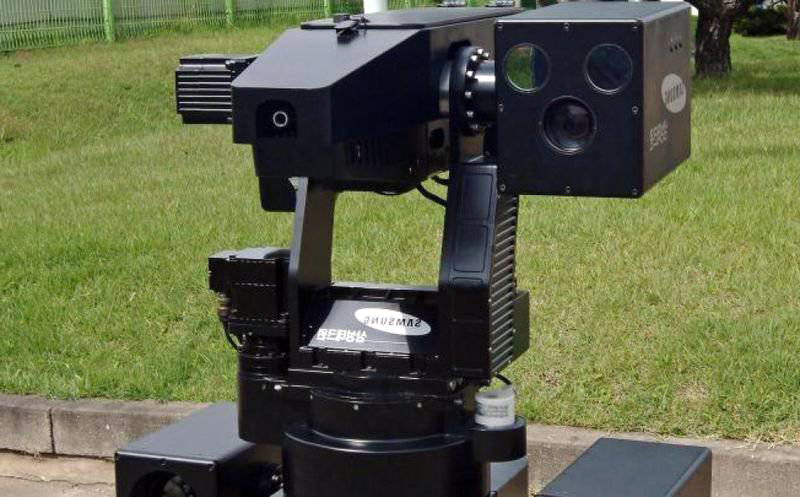
\includegraphics[scale=0.3]{./EtapaModerna/Imagenes/SGR-A1.jpg}
  	\caption{SGR-A1 (\href{https://commons.wikimedia.org/wiki/File:SGR-A1.jpg}{Wikimedia})}
  	\label{fig:sgra1}
  \end{figure}
\end{enumerate}

Como podemos ver en el ámbito de la industria militar se han desarrollado enormemente las capacidades de movilidad de los robots tanto aéreamente como de forma terrestre con lo que ello conlleva en los sistemas de cámaras y comunicación con los mismos.

\subsubsection{Avances de la IA}
Como hemos podido ver la Inteligencia Artificial ha acompañado a todos los modelos que hemos ido viendo a lo largo de la historia moderna de la robótica por lo que, lo presentado en esta sección, no va a estar alejado del resto de los apartados pero sí podemos destacar algunas de las intervenciones de la IA en algunos campos concretos en los que se han logrado grandes avances.

\vspace{10px}

Para analizar estos avances vamos a dividir la sección en diferentes temáticas relacionadas con aplicaciones reales para contextualizarlos:

\begin{enumerate}
  \item Salud: En el ámbito de la salud se han realizado muchas contribuciones en el tema debido a la complejidad a la hora de abordar la detección de enfermedades. Este hecho no es algo trivial ni mucho menos y, aunque el médico esté muy bien formado y tenga experiencia, no estamos seguros de que éste se confunda en el diagnóstico. Por ello algunas herramientas muy útiles (diseñadas por ejemplo por Microsoft) son las que aprenden sobre las enfermedades para ayudar al médico a reconocerlas y escoger el tratamiento más efectivo para la misma. En este ámbito podemos destacar las adaptaciones que sufrió el Watson de IBM para aprender sobre las enfermedades y poder contestar a preguntas de los médicos. En el tema sanitario también se están haciendo muchos avances en lograr un sistema robótico que facilite las tareas en el quirófano como por ejemplo un brazo robótico de alta precisión que ayude al cirujano en la misma. Incluso se planea que en un futuro las operaciones se puedan realizar de forma autónoma por robots siendo supervisados por médicos para poder detenerlos si cometen algún fallo durante el proceso.
  \item Automoción: en el ámbito de la automoción no es difícil imaginar los avances que la Inteligencia Artificial ha logrado con compañías como por ejemplo Tesla, Mercedes o Google. En este sentido tenemos dos objetivos actualmente en el sector: facilitar la conducción y sustituir al piloto. En el primer caso tenemos el ejemplo de compañías como Tesla o Mercedes que han incorporado los sistemas llamados Autopilot en los que el coche es capaz de analizar el entorno con el tráfico y las señales pudiendo operarse por él mismo fijando un destino en el sistema GPS incluido en el propio coche. En este tipo de avances ha sido muy importante el desarrollo de la visión por computador y la detección de señales y vehículos. Además este hecho no es trivial, puesto que en las decisiones que se le piden tomar a la máquina se incluyen dilemas que pertenecen más al ámbito de lo ético y moral que de lo puramente técnico. Por ejemplo, qué sería preferible: ¿atropellar a los tres peatones que están cruzando la calle con el semáforo en rojo o atropellar a un peatón inocente que está en la acera al intentar esquivar a los que cruzan? En el segundo punto, el de la sustitución del conductor, tenemos a compañías como Google o Apple que están liderando proyectos que ya son capaces de operar de forma completamente autónomas y están siendo refinadas. Además este sector se enfrenta a una regulación de los vehículos sin conductor a la que se tendrán que adaptar puesto que de momento, al ser la tecnología muy reciente, los países se encuentran reticentes a dejar a estos coche circular libremente por las ciudades.
  \item Economía: actualmente los bancos, bolsas y agentes financieros en general están constantemente haciendo uso de la IA tanto para predecir los movimientos del mercado como para hacer un análisis constante de las operaciones en tiempo real y poder aprender de ellas. No es raro que los bancos quieran obtener información de los usuarios (pues les reporta un gran beneficio a costa de los mismos) y para ello emplean técnicas muy avanzadas de predicción de movimientos financieros y categorización del nivel económico de las personas en función del tipo de operaciones que realizan. También, en este sentido, se están empleando programas que usan la inteligencia artificial para intentar tomar la mejor decisión en cada momento en para realizar inversiones en bolsa o comprar empresas pero este tipo de programas están siendo legislados ya que, por la rapidez de su toma de decisiones, ninguna persona podría competir contra este tipo de programas.
  \item Publicidad: en cuanto al tema publicitario las empresas que se encargan de gestionar los anuncios y la atracción de los clientes usan de forma constante los datos que los mismos generan para obtener información relevante para anunciar sus productos. Esto no sólo es aplicable a productos comerciales, si no que por ejemplo podría ser aplicable también a partidos políticos, los cuales podrían estudiar cuál es la mejor forma de hacer ``engagement'' con sus posibles votantes. En este ámbito del uso de la Inteligencia Artificial debemos de ser cuidadosos pues estamos traspasando la línea de lo que podría considerarse incluso como manipulación.
\end{enumerate}

Hemos visto en estos ejemplos que la IA puede ser de una utilidad enorme para la humanidad por la gran versatilidad que tiene, al poder aplicarse a una variedad enorme de temas, pero tenemos que tener en cuenta que esta herramienta puede llegar a ser un peligro si no se usara de forma correcta. En este ámbito podríamos poner lo que se conoce como Ingeniería Social (un eufemismo de manipulación) en la cual la IA nos podría dar una forma de obtener información de las personas, extraer conocimiento de dicha información y acabar manipulando al sujeto para que, por ejemplo, vote al partido político que nos interese. Debemos de valorar el potencial que tenemos con este tipo de herramientas pero sin despegarnos del hecho de que siempre se pueden utilizar de forma malintencionada.

\subsubsection{Robots humanoides}
Una de las fantasías y sueños del hombre ha sido el de poder crear un robot que imitara tan fielmente el comportamiento de un humano que nos pasara desapercibido como tal. Ene este terreno, Turing por ejemplo pensó en un test que delimitaba (o eso pensaba él) la frontera a partir de la cual un robot y una persona son indistinguibles. En este sentido hemos avanzado enormemente con robots como los ya visto tales como los primeros WABOT con forma humana hasta los ASIMO. Entramos ahora en un terreno mucho más avanzado en el que empezamos a hablar de posturas faciales e incluso de sentimientos y estados de ánimo.

\vspace{10px}

A continuación vamos a describir los robots que han representado un mayor avance o una mayor innovación en este terreno:
\begin{enumerate}
  \item Actroid: este robot fue diseñado en la universidad de Osaka y revelado en el año 2003. Hasta ahora, hemos explicado como los robots imitaban la forma de andar y comportarse de las personas, pero si observamos imágenes de los citados hasta el momento veremos que el parecido con los humanos no es para nada sorprendente. Este robot es el primero que mencionamos que realmente supone un salto en apariencia física, ya que es realmente parecido a un humano. El robot intenta no sólo parecerse físicamente, si no que también intenta que los movimientos que realiza sean lo más naturales y parecidos a los que podríamos hacer nosotros. El recubrimiento del robot está hecho de silicona intentando imitar la textura y consistencia de la piel. Además el robot actúa por él solo mediante el reconocimiento del terreno para intentar tener una interacción gestual adecuada con las personas. El punto más pobre de este diseño fue la asistencia por voz, la cual sólo implementaba un módulo de conversaciones sencillas que no permitían llevar una conversación fluida.
  \begin{figure}[!h]
  	\centering
  	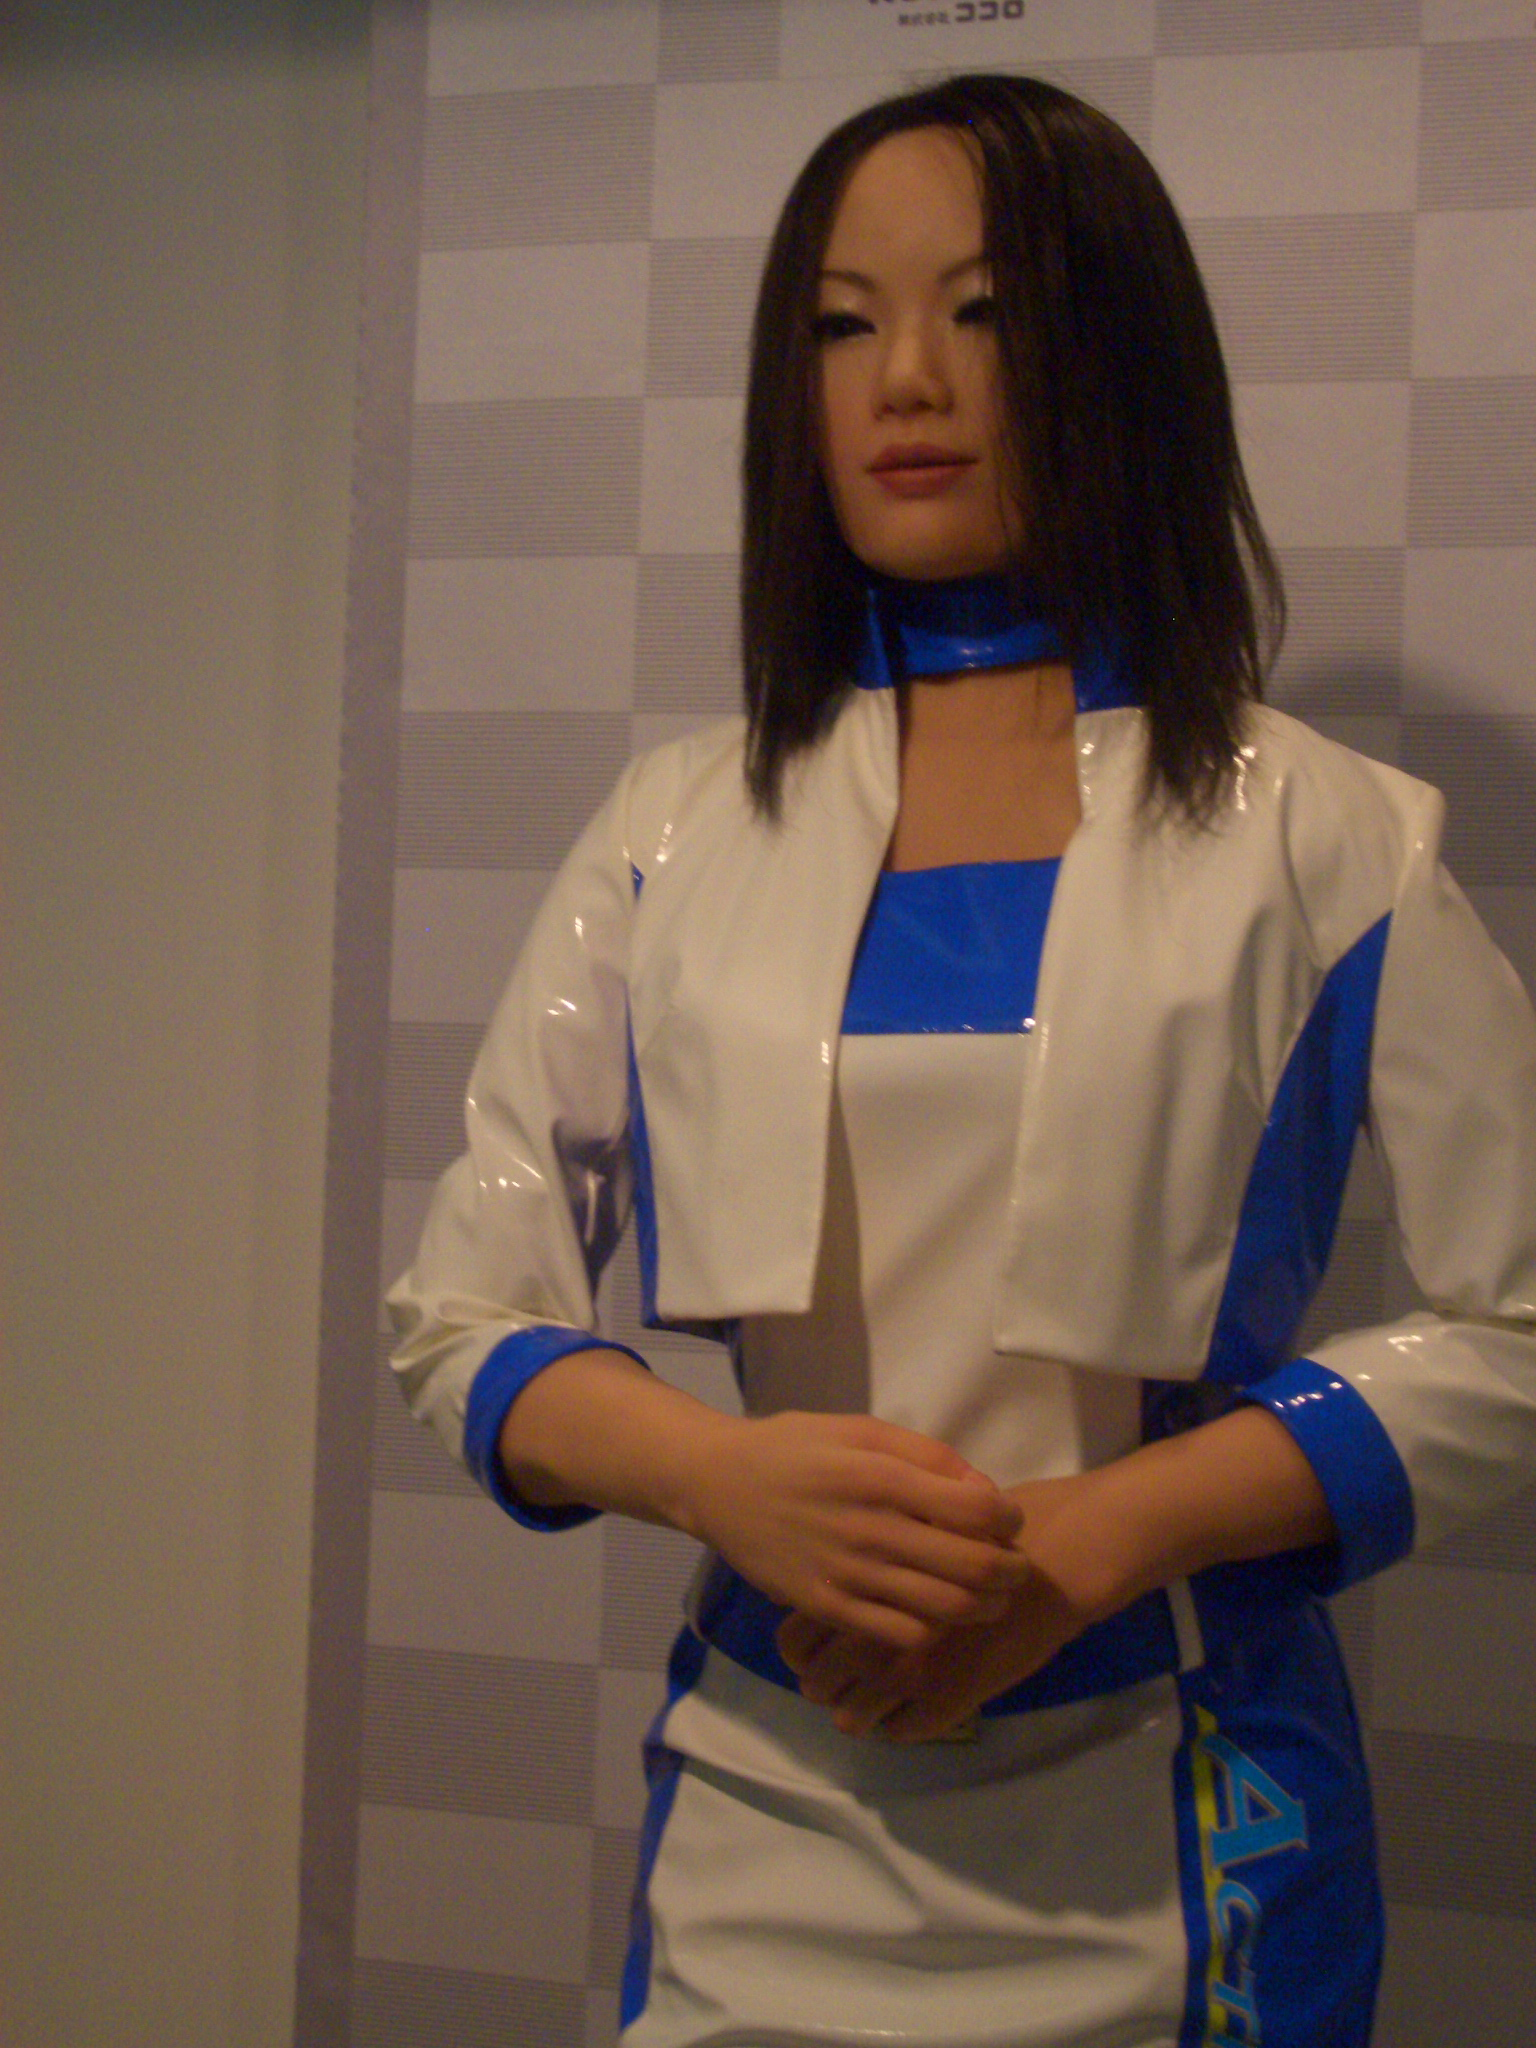
\includegraphics[scale=0.1]{./EtapaModerna/Imagenes/actroid.jpg}
  	\caption{Actroid (\href{https://commons.wikimedia.org/wiki/File:Actroid_3.jpg}{Wikimedia})}
  	\label{fig:actroid}
  \end{figure}
  \item Wakamaru: en el terreno justo complementario a Actroid había compañías como Mitsubishi Heavy Industries (parte del grupo Mitsubishi) que apostaban no sólo por la creación de robots con un parecido humano razonable, si no también por una interfaz conversacional más completa. Wakamaru fue sacado al mercado en el año 2005 con el propósito de poder interactuar con las personas de forma hablada. Sólo fue programado para reconocer el idioma Japonés siendo capaz de reconocer hasta 10.000 palabras. El robot estaba conectado a Internet para poder responder las consultas del usuario como por ejemplo el tiempo o algún dato que requiriera de búsquedas en Internet. El robot era capaz de desplazarse en superficies sencillas como las que podemos encontrar en una casa (sin incluir escaleras) para lo cual incorpora un sistema de cámaras para detectar el entorno. El robot funciona mediante una batería que le da una autonomía de 2 horas moviéndose él solo hasta su estación de carga cuando su batería está baja. El robot fue ampliamente criticado debido a que su precio rondaba los 15.000 dólares, lo cual es un precio realmente alto para una interfaz conversacional que anda.
  \begin{figure}[!h]
  	\centering
  	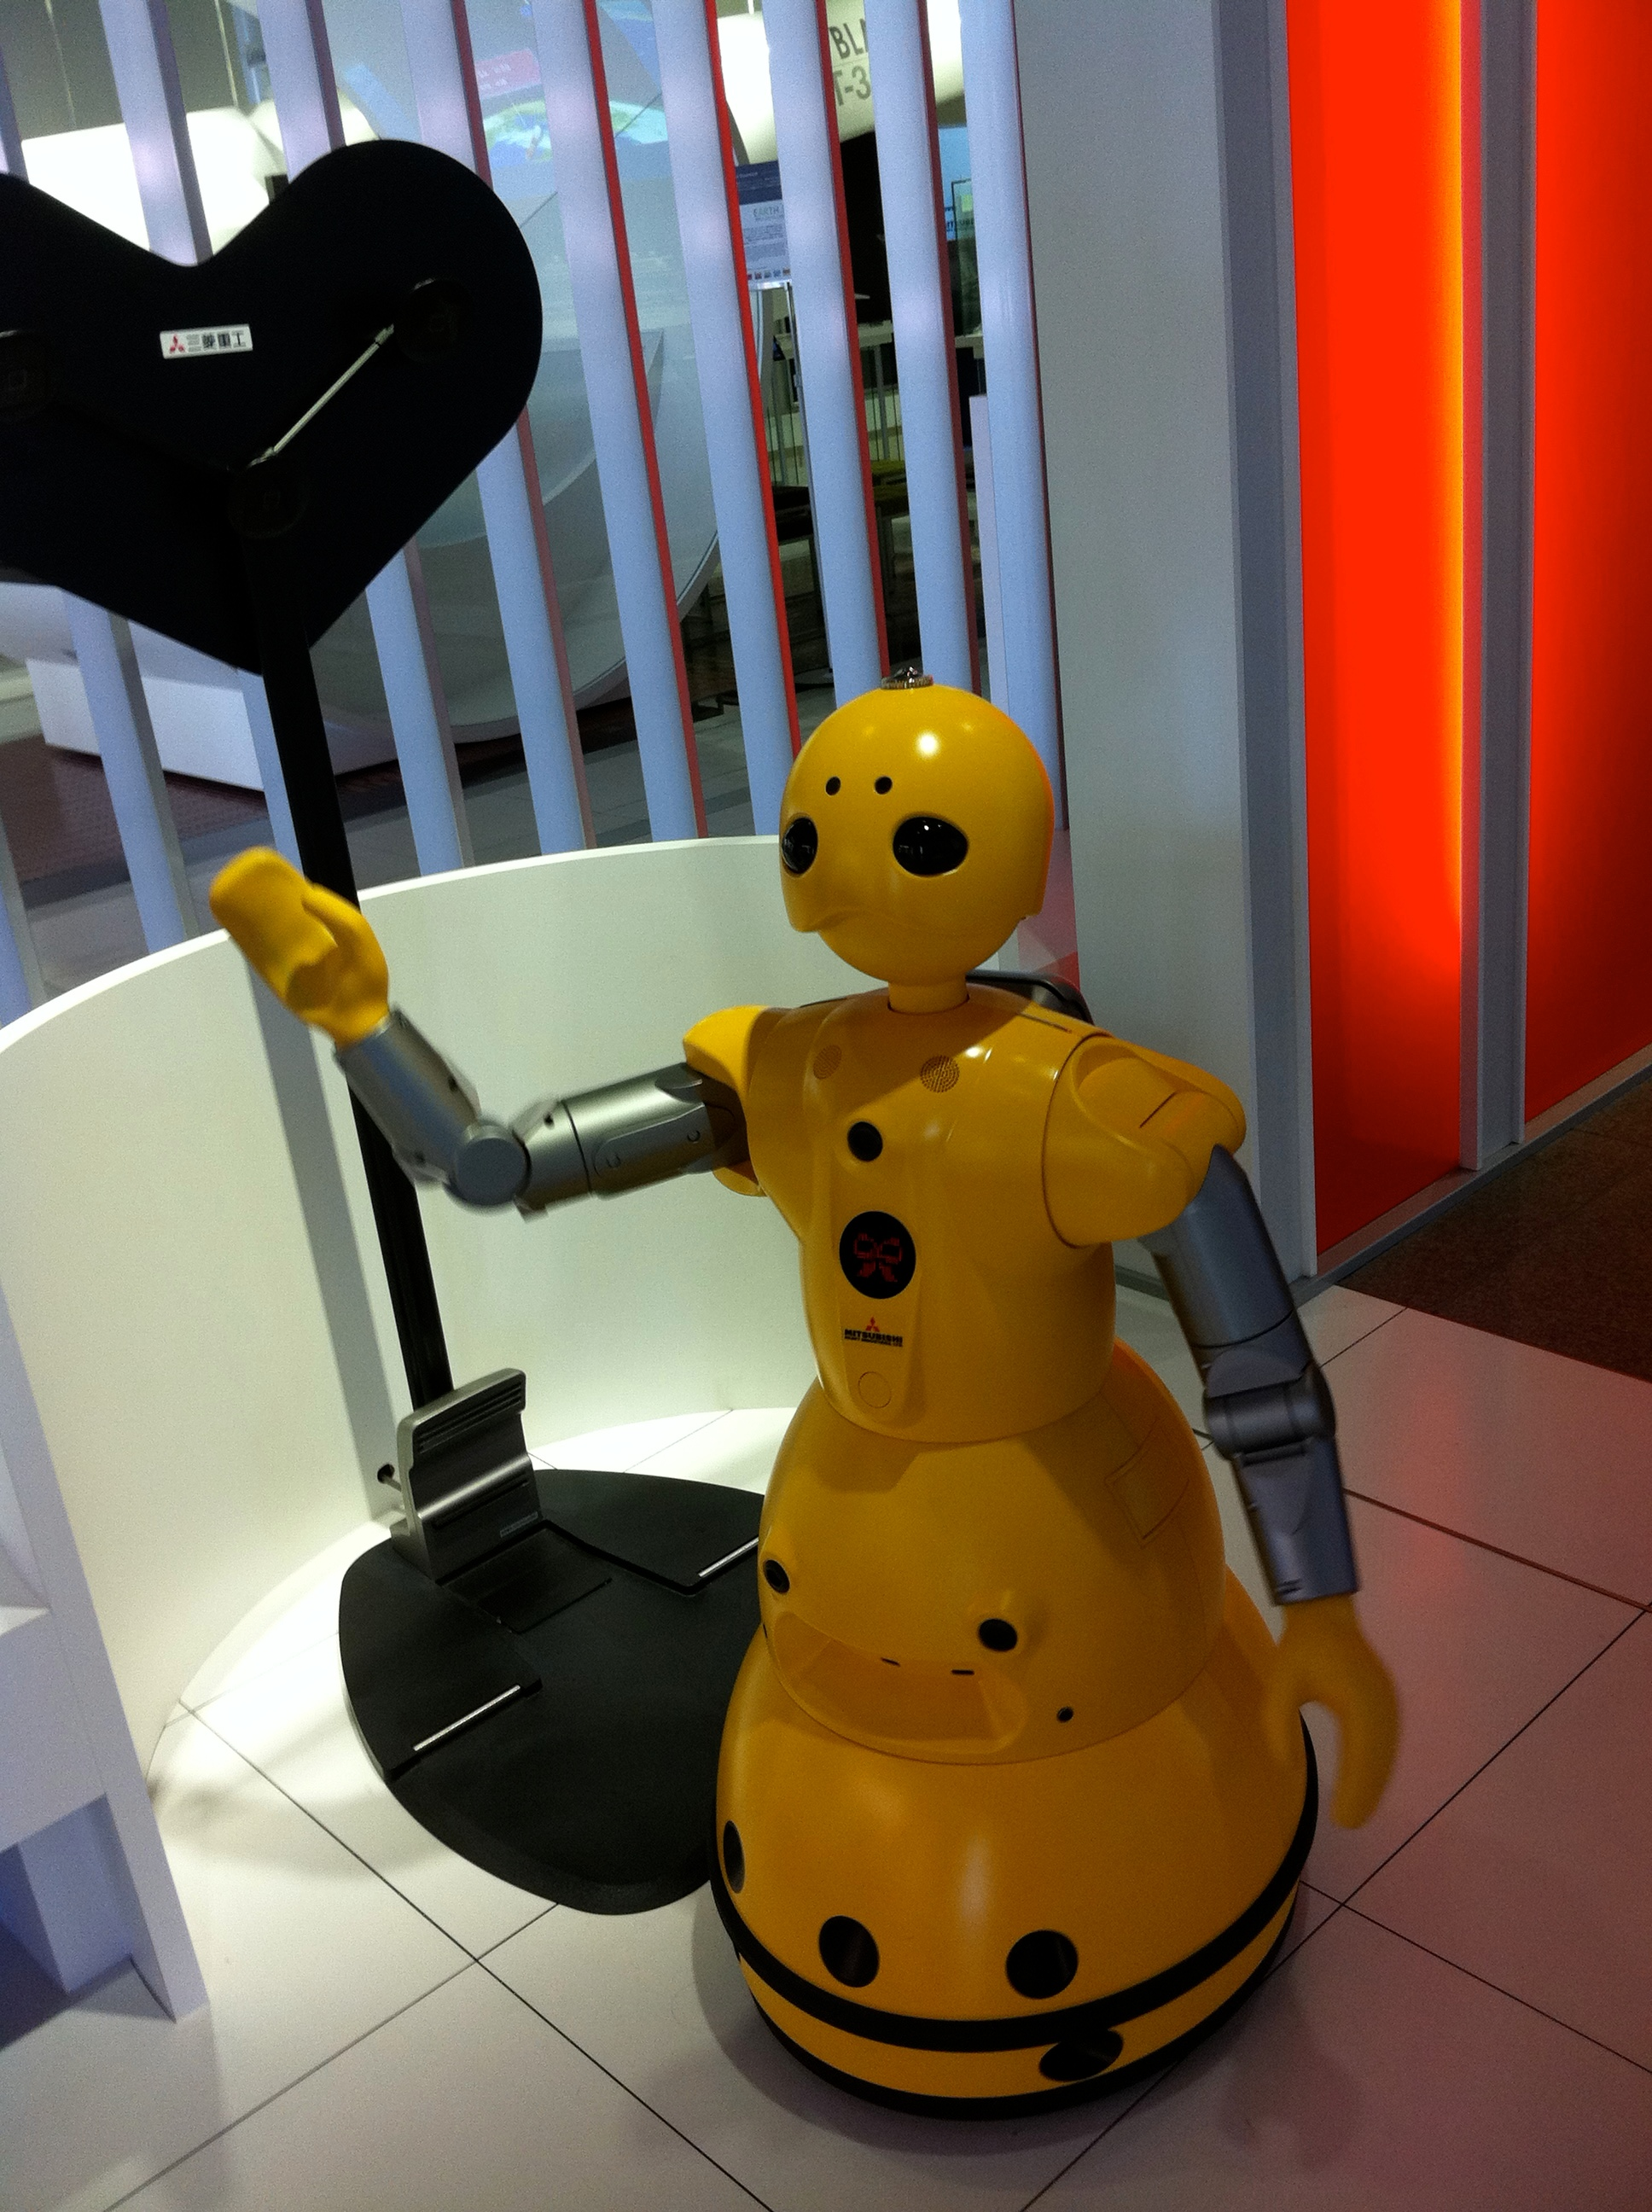
\includegraphics[scale=0.1]{./EtapaModerna/Imagenes/wakamaru.jpg}
  	\caption{Wakamaru (\href{https://commons.wikimedia.org/wiki/File:Wakamaru-fullshot2011.jpg}{Wikimedia})}
  	\label{fig:wakamaru}
  \end{figure}
  \item iCub: un paso más adelante en el terreno de los robots humanoides ha sido el robot iCub desarrollado por un conglomerado de Universidades europeas llamado RobotCup Consortium. El robot tiene el tamaño de un niño de unos tres años de edad. El robot incorpora unas articulaciones complejas con un sistema de tendones como nuestras propias articulaciones de forma que, bajo la percepción humana, el movimiento sería más realista. El robot fue un proyecto que intentaba ver cómo de precisa podía ser la imitación de los movimientos humanos complejos. Se consiguió que el robot se arrastrase, resolviera puzles tridimensionales complejos, practicó tiro con arco y cómo apuntar al centro de la diana analizando el entorno, imitación de las expresiones fáciles, control de fuerza y fue capaz de esquivar obstáculos de forma dinámica, esto es, esquivar los obstáculos conforme aparecen.
  \begin{figure}[!h]
  	\centering
  	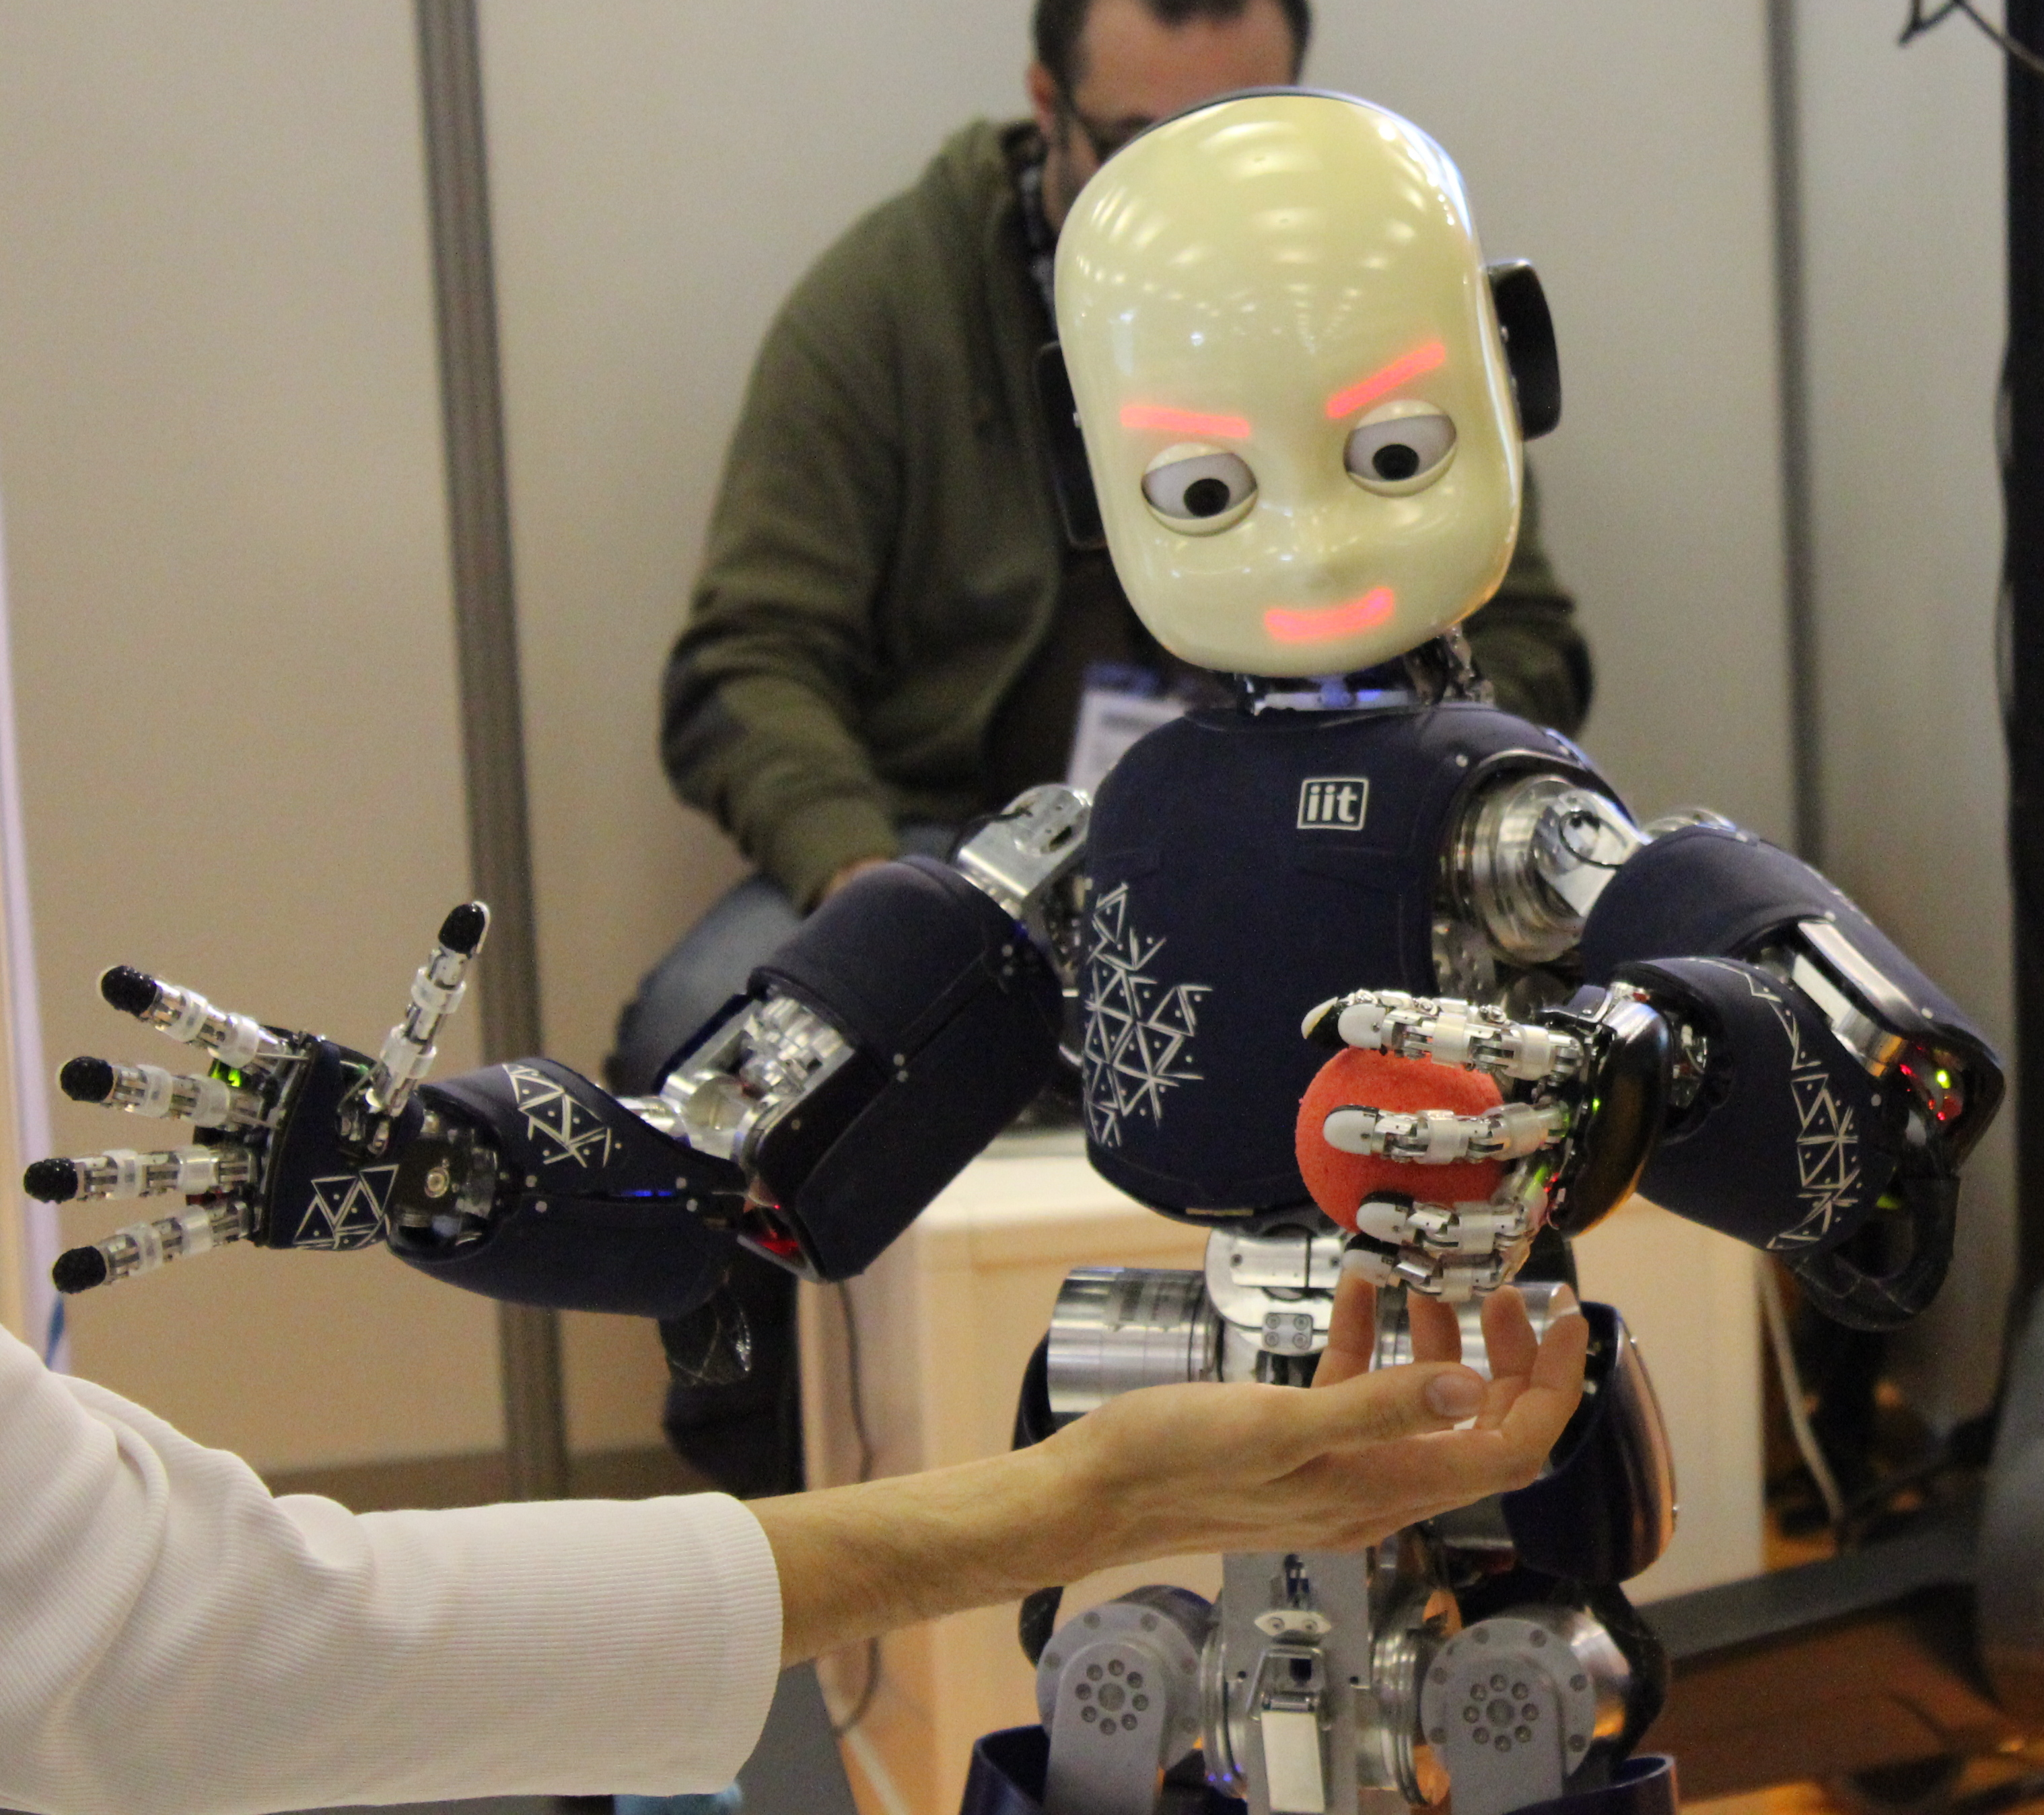
\includegraphics[scale=0.07]{./EtapaModerna/Imagenes/icub.JPG}
  	\caption{iCub (\href{https://commons.wikimedia.org/wiki/File:ICub_Innorobo_Lyon_2014.JPG}{Wikimedia})}
  	\label{fig:icub}
  \end{figure}
  \newpage
  \item Sophia: En el terreno de los robots humanoides este es el que actualmente lidera el ranking tanto de parecido humano físico como de capacidad de interacción oral y gestual. Sophia fue desarrollada por Hanson Robotics y se activó en 2016. Las cámaras que el robot incorpora están localizadas en sus ojos, de forma que la percepción de la realidad es la misma que la que podemos percibir los humanos. El primer modelo de Sophia sólo era un torso que demostraba la capacidad del robot de imitar los gestos y cambiar la expresión facial en función de su interlocutor y la conversación así como sus propias capacidades conversacionales. Este torso fue actualizado en enero de 2018 añadiéndole también unas piernas. El robot incorpora el sistema de reconocimiento de voz desarrollado por Alphabet con lo que implementa un reconocimiento muy completo y preciso. Las capacidades conversacionales de Sophia han sido ampliamente demostradas en muchas entrevistas con preguntas complejas sobre cualquier temática en las que Sophia ha sido capaz de responder de una forma muy elaborada y con sentido dentro de la conversación. Actualmente el desarrollo de Sophia sigue en pie añadiendo funcionalidades y mejorando las ya existentes.
  \begin{figure}[!h]
  	\centering
  	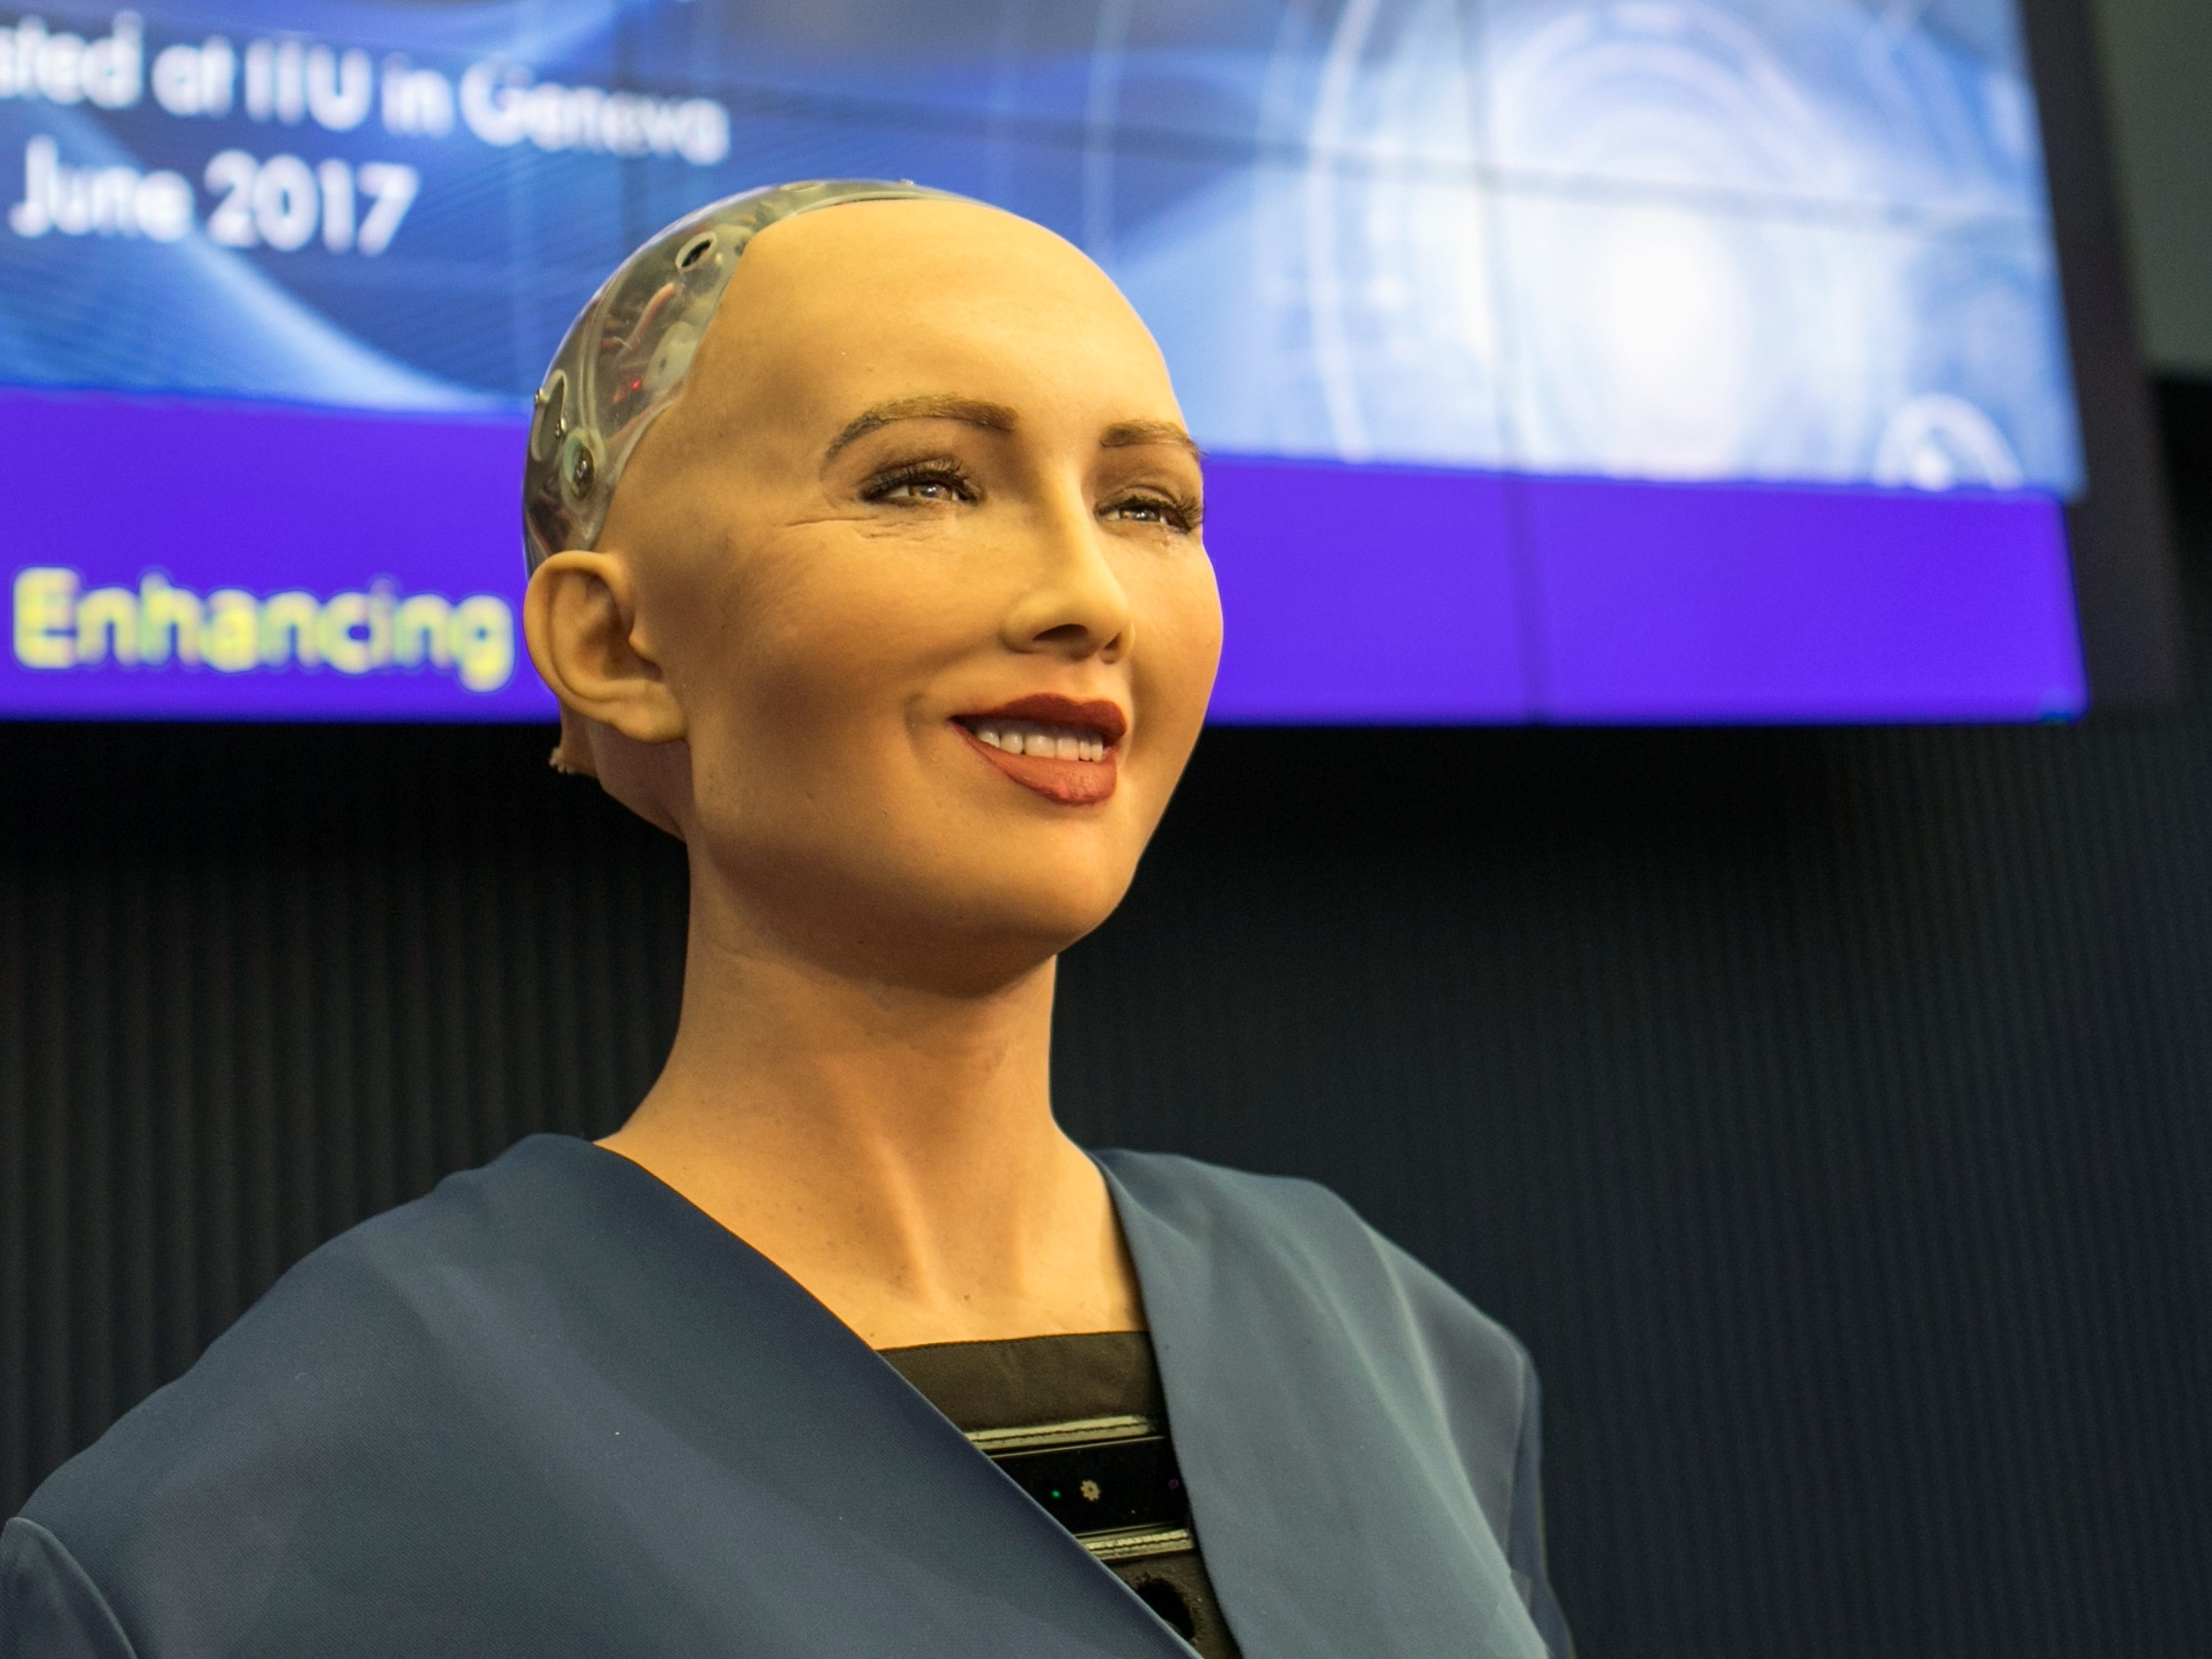
\includegraphics[scale=0.4]{./EtapaModerna/Imagenes/sophia.jpg}
  	\caption{Sophia (\href{https://es.wikipedia.org/wiki/Archivo:Sophia_(robot).jpg}{Wikimedia})}
  	\label{fig:sophia}
  \end{figure}
\end{enumerate}
